\section{Analytical Modeling}
In the previous section we studied the possibility of using a polynomial regression model to capture the relationship between grain size, number of cores, and throughput for a fixed matrix size, with the purpose of finding a range of grain size that leads us to maximum performance. 
Although the polynomial function was helpful in directing us toward our objective of finding the region of grain size with maximum performance, it lacked a physical implication, and was not quite able to capture the overall behavior of the system. 

This motivated us to change our view, and instead of looking just at the data and trying to find a function to fit the data, study the behavior of the data, and then find a function that would be likely to fit and explain the data. That function would be a good fit mostly because that's how we expect the throughput to change with grain size, and not solely how the data behaves.   

In this chapter we attempt to understand the effect of grain size on the achievable speedup in an asynchronous many-task runtime system, in order to develop an analytical model for predicting the execution time in an asynchronous many task runtime system. 

We have to note here that even if we were able to identify all the factors affecting the execution time, it is still very hard to find an analytical model describing the relationship between these factors and the execution time. In this chapter we explain our effort in this direction by starting from a simple benchmark. We suggest a formula based on our knowledge of the behavior of the system, and the collected data. Then we will try to generalize the proposed formula to arbitrary parallel for-loops with balanced work-load for each iteration. 


Throughout this chapter we will be using the following terms and definitions to simplify our work. We represent the number of cores available with $N$, the number of tasks created as $num\_{tasks}$, the maximum amount of work assigned to one core as $w\_c$, the number of cores that are actually doing the work(when there is not enough work for all the cores) as $M$ ($M\leq{N}$), the total amount of work available as $problem\_{size}$, and the sequential execution time as $t\_{seq}$.

In an attempt to find this analytical model for execution time of a balanced parallel for-loop, we started with looking into two factors that we believe play the most important role in determining the execution time: the overhead of creating tasks, and the maximum amount of work assigned to one core. 

In order to understand how these factors contribute to the execution time in a balanced parallel for-loop, we define \emph{iter\textunderscore{length}} as the amount of time to execute one iteration, \emph{num \textunderscore{iterations}} as total number of iterations, $chunk\_{size}$ as number of iterations to be executed by one thread.


The total execution time could be assumed to be roughly the amount of time it takes for the core with the maximum amount of work to finish it's job. Here we call the core with maximum expected amount of work as $core_0$, and the associated amount of work as $w\_c$. 
With this assumption, the main factors contributing to the execution time are the overhead of creating and managing tasks on $core_0$, the time it takes to run $w\_c$ amount of work on $core_0$, denoted with $t\_{c}$, and the number of cores that will be executing the work($M$). Depending on the amount of work available, either all $N$ cores or less than $N$ cores will be performing the work.

Formula~\ref{formula31} shows the expected formula in it's simplest form.

\begin{equation}\label{formula31}
\begin{aligned}
&execution\_time = 
t\_{overhead}\:\:+\:\:t\_c\
\end{aligned}
\end{equation}


In Formula\ref{formula31}, $t\_{overhead}$ represents the penalty that we have to pay for running the program in parallel. We hold two major factors accountable for this overhead. 

The first factor is the overhead of creating and managing the tasks. Although this overhead is negligible for small number of tasks, it becomes significant as the number of created tasks becomes larger, playing an important role in the overall execution time.

When $num\_{tasks}$ tasks are created, $\left\lceil{\frac{num\_{tasks}}{N}}\right \rceil$ tasks would be created on $core\_0$. If we represent the overhead of creating and managing a task on one core with $\alpha$, the portion of $t\_{overhead}$ resulted from $num\_{tasks}$ tasks could be stated as $\alpha\times{\left\lceil{\frac{num\_{tasks}}{N}}\right \rceil}$.

%The second factor is the overhead of managing the created tasks. While the overhead of creating a task should be constant on a specific machine architecture, we are suggesting here that the overall overhead of managing $num\_{tasks}$ tasks, is a factor($\delta$) of $N$. This effect is originated from HPX's strategy to avoid allocating new stacks by keeping the previous stack alive until new thread is created, at that point the stack is assigned to the new thread. 
%The overhead of managing a task on a machine is shown with $\delta\times{num\_{tasks}}$.

The second factor is the overhead caused by work stealing. Although work stealing is a very helpful method for load balancing, it induces an overhead due to constant efforts of idle cores to steal work from the other cores. Each of these efforts would result in trashing the local cache of the busy cores. This effect helps for load balancing when the number of tasks created is greater than or equal to the number of cores, but as the number of tasks get smaller than the number of cores, the unsuccessful steal efforts become more noticeable.

HPX by default uses the priority local scheduling policy which creates one queue for each core. When there is no more work left in one core's queue, it will attempt to steal work from other cores starting from it's neighbors. If the attempt is not successful, it will move on to the next level neighbors. This continues until the core that initiates the steals(called the thief) is able to find a core with tasks in their queue which can be stolen(called the victim). 

HPX provides an optional command line parameter ${--hpx:numa-sensitive}$ to make sure that the thief would try the queues of the cores in the same NUMA domain first. This option is provided based on the fact that it is much faster to access the local memory of a processor than the local memory of another processor.  
%In our example we are only using 8 cores from the same NUMA domain 

Expressing the total overhead as the summation of the overhead of creating and managing the tasks, and the overhead resulted from work stealing, as shown in Formula~\ref{formula33},
 
\begin{equation}\label{formula33}  
\begin{aligned}
t_{overhead}=\alpha\times{\left\lceil{\frac{num\_{tasks}}{N}}\right\rceil}\:\:+\:\:t\_{overhead\_{ws}}
\end{aligned}
\end{equation}

Formula~\ref{formula31} then becomes:

\begin{equation}\label{formula32}
\begin{aligned}
&execution\_time = 
\alpha\times{\left\lceil{\frac{num\_{tasks}}{N}}\right\rceil\:\:+\:\:t\_{overhead\_{ws}}\:\:+\:\:t\_c}
\end{aligned}
\end{equation}

We had previously defined $t\_c$ as the time it takes to perform $w\_c$ amount of work, where $w\_c$ is the maximum amount of work assigned to the cores. 

For a balanced parallel for-loop, $w\_c$ can be calculated as:
\vspace{\baselineskip} 
\begin{equation}\label{formula2}
w\_c =\left\{
\begin{aligned}
&problem\_{size} \:\:\:\:\:\:\:\:\:\:\:\:\text{ if } N=1\\
&problem\_{size}-g\times{(N-1)}\times(\left \lceil{\frac{num\_{tasks}}{N}}\right \rceil-1) \\
&\:\:\:\:\:\:\:\:\:\:\:\:\:\:\:\:\text{if }num\_{tasks}\%N=1\text{\:\:\&\:\: }num\_{iterations}\%chunk\_{size}\neq0\\ 
%\text{\:\:or} \\ g\times(\left \lceil{\frac{num\_{tasks}}{M}}\right \rceil-1)+(num\_{iterations}\%chunk\_{size})\times(iter\_{length}) \\ \:\:\:\:\:\:\:\:       
&g\times\left \lceil{\frac{num\_{tasks}}{N}}\right \rceil  \:\:\:\:\:\:\:\:\:\:    \text{otherwise}
\end{aligned}
\right.
\end{equation}
\vspace{\baselineskip}

When $N=1$, all the work will be assigned to the only available core, causing $w\_c$ to be equal to all the available work, $problem\_{size}$.

When $N>1$, in the general case at most $\left \lceil{\frac{num\_{tasks}}{N}}\right \rceil$ tasks would be assigned to a core. Therefore, with a grain size of $g$ each task would contain $g$ amount of work, resulting in a maximum amount of work of $g\times{\left \lceil{\frac{num\_{tasks}}{N}}\right \rceil}$ assigned to a core.

It should be noted that the last chunk of work created could contain less amount of work than the $chunk_size$, and this is the case when $num\_{iterations}\%chunk\_{size}\neq0$. This although causing less amount of work to be assigned to one of the cores, would not affect the maximum amount of work assigned to the cores, unless when $num\_{tasks}\%N=1$. For these special cases where $num\_{tasks}\%N=1$ and  $num\_{iterations}\%chunk\_{size}\neq0$ the maximum amount of work assigned to the cores would be $problem\_{size}-g\times{(N-1)}\times(\left \lceil{\frac{num\_{tasks}}{N}}\right \rceil-1)$. 

Figure~\ref{fig58} illustrates how $w\_c$ is calculated for this case. Each square represents a chunk or one task, containing $g$ amount of work generating $num\_{tasks}$ chunks in total, and each column represents one core. The last chunk contains $g'=num\_{iterations}\%chunk\_{size}$ amount of work, where $g'<g$ and $g\times{(N)}\times(\left \lceil{\frac{num\_{tasks}}{N}}\right \rceil-1)+g'=problem\_{size}$.

\begin{figure}[H]
	\centering
	{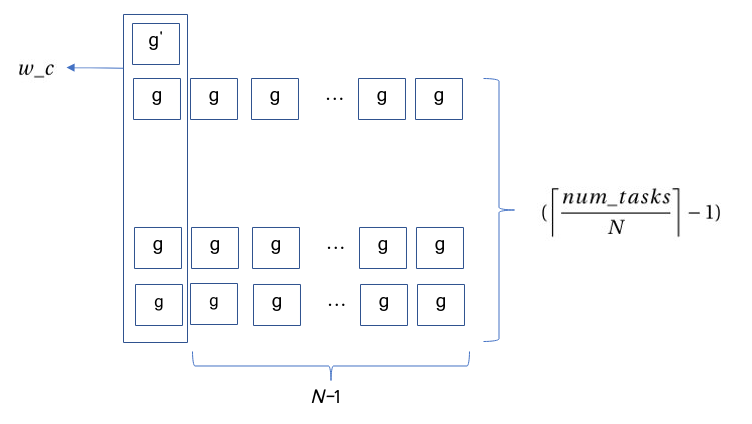
\includegraphics[scale=.3]{images/w_c_explained.png}}
	\caption{The way $w\_c$ is calculated illustrated for cases where $num\_{tasks}\%N=1$ and  $num\_{iterations}\%chunk\_{size}\neq0$.}\label{fig58}		
\end{figure}

%On the other hand, when number of tasks created is smaller than the number of cores, we observe continuous efforts from the idle cores to steal work from cores that are actually doing the work, interrupting the cache coherency constantly. We represent this effect with $\delta\times{(N-M)\times{M}}\times{num\_{tasks}}\times{\frac{1}{M}})$.

  

%\begin{equation}\label{formula1}
%\begin{aligned}
%&execution\_time = \\
%\left\{
%\begin{aligned}
%&
%\alpha\left\lceil{\frac{num\_{tasks}}{M}}\right \rceil +\beta\times{(N-1)}{num\_{tasks}}+{w\_c+\sigma\times{w\_c}\times{(M-1)}} \:\: \text{if\:\:}num\_{tasks}>N\\
%&\alpha\left \lceil{\frac{num\_{tasks}}{M}}\right \rceil +\delta\times\frac{num\_{tasks}-1}{N}+{w\_c+\sigma\times{w\_c}\times{(M-1)}} \:\: \text{otherwise}
%\end{aligned}
%\right.
%\end{aligned}
%\end{equation}
\vspace{\baselineskip}

As discussed in chapter~\ref{Background}, Amdahl's law and Universal Scalibility Law suggest that for a fixed problem size, as we increase the number of cores in a multi-core system, the observed speedup is less than the linear speedup. which is mainly resulted from latency and coherency.
Universal Scalibilty Law\cite{gunther2007guerrilla} suggests that an overhead associated with the number of cores should be added to the expected execution time. Formula~\ref{formula16} shows the effect of contention($\sigma$) and coherency($\kappa$) in the overall execution time, with sequential execution time of $t_s$, on $N$ cores.

\begin{equation}\label{formula16}
\begin{aligned}
 &speed\-up\:\:=\:\:\frac{t_s}{t}\:\:=\:\:\frac{N}{1+\sigma\times{(N-1)}+\kappa\times{N(N-1)}}\Rightarrow\\
 &t\:\:=\:\:\frac{t_s}{N}\:\:+\:\:\sigma\times{(N-1)}\frac{t_s}{N}\:\:+\:\:\kappa\times{{N\times(N-1)}\frac{t_s}{N}} 
\end{aligned}
\end{equation}
\vspace{\baselineskip}

Formula~\ref{formula16} shows how USL models the overheads due to contention and coherency in execution time, when $\frac{t_s}{N}$ is the expected execution time on $N$ cores in ideal case when the mentioned overheads did not exist.

Based on Formula~\ref{formula16}, we added the term $\sigma\times(N-1)\times{t_c}$ to Formula~\ref{formula32} to represent the overhead observed due to contention effect, assuming $t_c$ is the ideal execution time in this problem. We ignored the overhead due to coherency since we do not expect to experience any inter-process communication overheads in this problem.

\begin{equation}\label{formula34}
\begin{aligned}
&execution\_time = 
\alpha\times{\left\lceil{\frac{num\_{tasks}}{N}}\right\rceil\:\:+\:\:t\_{overhead\_{ws}}\:\:+\:\:t\_c\:\:+\:\:t\_c\times{\sigma\times(N-1)}}
\end{aligned}
\end{equation}
%\vspace{\baselineskip}
 
Moreover, we adjusted Formula~\ref{formula34} by changing the total number of cores ($N$) to the number of cores that are actually executing the work ($M$), since there are cases where there is not enough work for all the cores to execute, and we expect the overheads due to contention to be a factor of the cores that are actually performing the work and not just all the cores.

Assuming that we are running our application on $N$ cores, with a grain size equal to $g$, $num\_{tasks}$ tasks are being created, and $M$ cores are actually doing the work. If $num\_{tasks}<N$, $M$ would be equal to $num\_{tasks}$, otherwise $M=N$.

\begin{equation}\label{formula19}
M=\left\{
\begin{aligned}
&num\_{tasks} \text{\:\:\:\:if \:} num\_{tasks}<N\\
&N \text{\:\:\:\:otherwise}
\end{aligned}
\right.
\end{equation}


Formula~\ref{formula34} is then converted into:

\begin{equation}\label{formula1}
\begin{aligned}
execution\_time = 
\alpha\times{\left\lceil{\frac{num\_{tasks}}{N}}\right\rceil}\:\:&+\:\:t\_c\:\:+\:\:\sigma\times{t\_c}\times{(M-1)}\:\:\\
&+\:\:t\_{overhead\_{ws}}
\end{aligned}
\end{equation}


As for $t\_{c}$, the time to execute $w\_{c}$ amount of work, where total amount of work available is $problem\_{size}$, since we are looking into balanced parallel for-loops with almost same amount of work at each iteration, we can estimate $t\_{c}$ as:

\begin{equation}\label{formula41}
\begin{aligned}
t\_{c}\:\:=\:\:t\_{seq}\times{\frac{w\_c}{problem\_{size}}}
\end{aligned}
\end{equation}

Where $t\_{seq}$ is the to run the whole amount of work, $problem\_{size}$ sequentially.

\begin{equation}\label{formula42}
\begin{aligned}
execution\_time = 
\alpha\times{\left\lceil{\frac{num\_{tasks}}{N}}\right\rceil}\:\:&+\:\:t\_{seq}\times{\frac{w\_c}{problem\_{size}}}\times{(1\:\:+\:\:\sigma\times{(M-1)})}\:\:\\
&+\:\:t\_{overhead\_{ws}}\\
\end{aligned}
\end{equation}


Here $t\_{overhead\_{ws}}$ represents all the overhead created due to work stealing. We did some investigations on where this term is originated from for a more precise modeling, but we were not successful. 

In order to study this effect, we ran a set of experiments while work stealing was turned of. This is possible through adding the command line option \emph{--hpx:queuing = static-priority}.

Figure~\ref{fig40} shows the results of running a benchmark with and without work stealing. The benchmark consists of a HPX parallel for-loop with $3000$ iterations and is executed with different number of chunk sizes from $1$ to $3000$. Each iteration will keep the core busy for $1\mu{sec}$. This benchmark is explained more in the next chapter.

As it can be observed, in the region where the number of tasks created is same as the number of cores, this effect is more significant.

\vspace{\baselineskip}	
\begin{figure}[H]
	\centering
	\subfloat[]{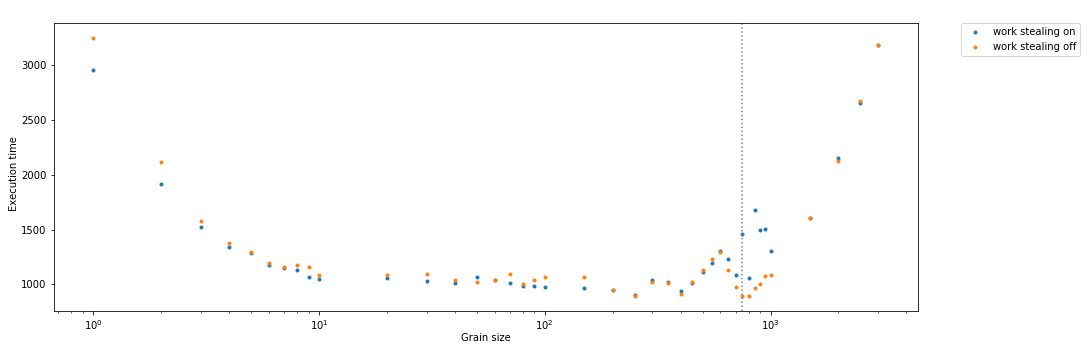
\includegraphics[scale=.4]{images/hpx_for_loop/3000_4_1_all.png}\label{fig40:a}}{\hfill}
	\subfloat[]{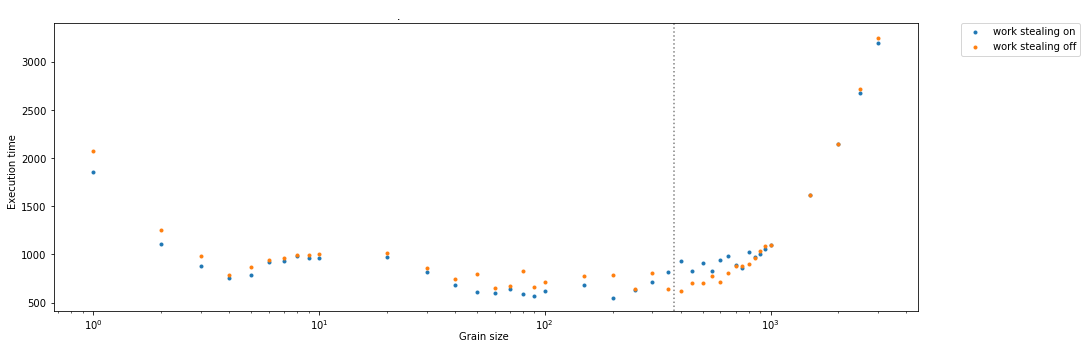
\includegraphics[scale=.4]{images/hpx_for_loop/3000_8_1_all.png}\label{fig40:b}}
	\caption{The results of running the parallel for-loop benchmark with $problem\_size=3000$, on different (a)4 cores, and (b) 8 cores. The vertical dotted line shows the grain size that would generate same number of tasks as the number of cores, with the same amount of work for all the cores.}\label{fig40}		
\end{figure}

Although we are not sure how work stealing is causing this effect, the effect is most  noticeable at certain points. Since it only adds to the execution time at those points, and our interest is finding the flat region of the graph with the minimum execution time, at this point and for this purpose we decided to ignore this term in our upcoming calculations. 

By ignoring the overhead caused by work stealing at this point, Formula~\ref{formula1} is simplified into Formula~\ref{formula7}, which will be referred to as our proposed analytical model in the next sections. 

\begin{equation}\label{formula7}
\begin{aligned}
execution\_time = 
\alpha\times{\left\lceil{\frac{num\_{tasks}}{N}}\right\rceil}\:\:&+\:\:t\_c\:\:+\:\:\sigma\times{t\_c}\times{(M-1)}\\
=\alpha\times{\left\lceil{\frac{num\_{tasks}}{N}}\right\rceil}\:\:&+\:\:t\_{seq}\times{\frac{w\_c}{problem\_{size}}}\times{(1\:\:+\:\:\sigma\times{(M-1)})}
\end{aligned}
\end{equation}

To summarize, we believe the important factors in determining the execution time in a balanced parallel for-loop are: number of tasks being created, number of cores the program is ran on, and the maximum amount of work one core has to perform. 

The maximum number of tasks assigned to one core, and the number of cores that are actually performing the work, are two other important factors that can be deducted from the aforementioned factors. 


\vspace{\baselineskip}
\subsection{Validating the Proposed Model}
In order to validate the proposed model, we created a benchmark based on a simple \textit{for\textunderscore{loop}} with different number of iterations, and chunk sizes, as shown in Listing~\ref{hpx_for_loop}. We refer to this benchmark as the parallel for-loop benchmark from now on.

Each iteration consists of a while loop that makes sure the iteration lasts a certain amount of time ($iter\_{length}$). By setting $iter\_{length}=1\mu{sec}$, and changing $num\_{iterations}$, and \emph{chunk\_{size}}, we can see how the execution time changes when the problem is executed on different number of cores. Having defined $problem\_{size}$ at the total amount of work that has to be performed, for this benchmark \textit{problem\textunderscore{size}} would be the time it takes to execute all the iterations, which is:

\begin{equation}\label{problem_size}
problem\_size = iter\_length\times{num\_iterations}
\end{equation}

Since we have set $iter\_{length}=1\mu{sec}$ in this benchmark, $problem\_size = num\_iterations$.
  
On the other hand, for this specific problem $t\_c=w\_c$ since there is no actual work happening  $t\_{seq}=problem\_{size}$ and $t\_c=w\_c$.
 
In order to test how well the suggested model in Formula~\ref{formula7} could fit the data for this problem, we collected a considerable amount of data (around 50,000 data points on three different architectures) with different configurations of number of cores($N$), number of iterations(\emph{num\_{iterations}}), and chunk size ($chunk\_{size}$).  

For each $num\_{iterations}$, we change the $chunk\_{size}$ from 1 to $num\_{iterations}$ in logarithmic scale. Each of these runs was executed for $N=1,2,3,...,8$.  

\begin{lstlisting}[basicstyle=\fontsize{8}{9}\selectfont,float,floatplacement=H,caption= {For-loop benchmark, a simple hpx for\textunderscore{loop} used to study the effect of grain size on the achieved parallelism.}, label={hpx_for_loop}]

///////////////////////////////////////////////////////////////////////////////
void measure_function_futures_for_loop(std::uint64_t count, bool csv, std::uint64_t chunk_size, std::uint64_t iter_length)
{
	// start the clock
	high_resolution_timer walltime;
	hpx::parallel::for_loop(hpx::parallel::execution::par.with(
	hpx::parallel::execution::dynamic_chunk_size( chunk_size )),
		0, count, [&](std::uint64_t) { worker_timed(iter_length*1000); });
	// stop the clock
	const double duration = walltime.elapsed();
	print_stats("for_loop", "par", "parallel_executor", count, duration, csv);
}

///////////////////////////////////////////////////////////////////////////////
int hpx_main(variables_map& vm)
{	
	const int repetitions = vm["repetitions"].as<int>();
	num_threads = hpx::get_num_worker_threads();
	const std::uint64_t chunk_size = vm["chunk_size"].as<std::uint64_t>();
	const std::uint64_t iter_length = vm["iter_length"].as<std::uint64_t>();
	const std::uint64_t count = vm["num_iterations"].as<std::uint64_t>();
	bool csv = vm.count("csv") != 0;
	if (HPX_UNLIKELY(0 == count))
		throw std::logic_error("error: count of 0 futures specified\n");
	for (int i = 0; i < repetitions; i++)
	{
		measure_function_futures_for_loop(count, csv, chunk_size, iter_length);
	}	
	return hpx::finalize();
}
///////////////////////////////////////////////////////////////////////////////
inline void worker_timed(std::uint64_t delay_ns)
{
	if (delay_ns == 0)
		return;
	std::uint64_t start = hpx::util::high_resolution_clock::now();
	while (true)
	{
		// Check if we've reached the specified delay.
		if ((hpx::util::high_resolution_clock::now() - start) >= delay_ns)
			break;
	}
}
///////////////////////////////////////////////////////////////////////////////
int main(int argc, char* argv[])
{
// Configure application-specific options.
	options_description cmdline("usage: " HPX_APPLICATION_STRING " [options]");
	cmdline.add_options()("num_iterations",
		value<std::uint64_t>()->default_value(500000), "number of iterations to invoke")
		("repetitions", value<int>()->default_value(1),
		"number of repetitions of the full benchmark")
		("iter_length",value<std::uint64_t>()->default_value(1), "length of each iteration")
		("chunk_size",value<std::uint64_t>()->default_value(1), "chunk size");
	// Initialize and run HPX.
	return init(cmdline, argc, argv);
}
\end{lstlisting}

%As an example, for $problem\_{size}=100000$, we have collected 64 data points for each $N=1,2,...,8$, resulting in $512$ data points in total. Figure~\ref{fig41} shows the execution time for different grain sizes ranging from 1 to 100000 for $problem\_{size}=100,000$ with $N=8$.

Figure~\ref{fig41} shows an example of the results obtained from running the parallel for-loop benchmark in Listing~\ref{hpx_for_loop}, for $problem\_size=100,000$, on 8 cores.
\begin{figure}[H]
	\centering
	{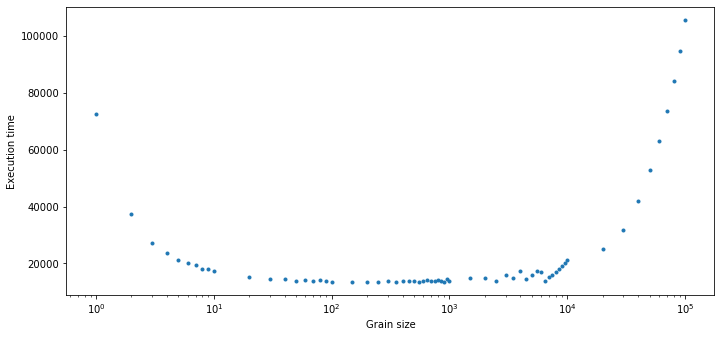
\includegraphics[scale=.45]{images/hpx_for_loop/100000_8.png}}
	\caption{The results of running the parallel for-loop benchmark with $problem\_size=100,000$, on 8 cores. The unit for execution time is microseconds.}\label{fig41}		
\end{figure}


%\vspace{\baselineskip}	
%\begin{figure}[H]
%	\centering
%	{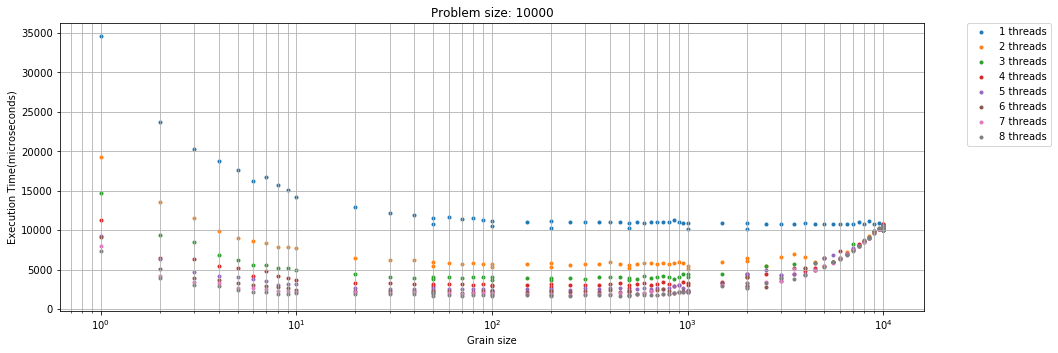
\includegraphics[scale=.45]{images/hpx_for_loop/10000_8_all.png}}
%	\caption{The results of running the benchmark in Listing with $problem\_size=10000$, on different number of cores.}\label{fig39}		
%\end{figure}

As stated in Chapter~\ref{Background}, the graph of execution time vs grain size looks like a bathtub curve, with three major regions we refer to as left hand side, right hand side, and the flat region of the graph. 

At the right hand side of the graph in with large grain sizes, the number of tasks created is smaller than the number of cores which results in making at least one of the cores idle, while the other cores are assigned a rather big chunk of work. The performance degradation we observe at those points is associated with starvation. Starvation refers to situations where we are not utilizing our computation resources to the full extent. At these points, the number of cores actually performing the work is equal to the number of tasks, since each core gets to execute at most one task. 

At this region of the graph, the time to execute the maximum assigned work to a core ($t\_c$) is the dominant factor in determining the execution time.   

On the other hand, on the left hand side of the graph with small grain sizes, we end up with creating a large number of tasks. Since there is an overhead associated with each created task, we observe a performance degradation in that region. As the grain size increases, the number of created tasks, and the overhead associated to that decreases consequently. At this region of the graph, the overhead of creating and managing the tasks is the dominant factor in determining the execution time.   

The third region of the graph, which we referred to as the flat region of the graph, is the area between the two mentioned areas where we observe very little change in the execution time. At this region, the overhead associated with creating and managing the tasks is amortized by the execution time and since all the cores are utilized we do not observe he effect a performance degradation due to starvation.

Our intention in this thesis is to find this flat region of the bathtub curve, as shown in Figure~\ref{fig60:a}, in order to ensure that the effect of the two major sources of performance degradation (overheads of creating and managing tasks, and starvation) in execution time is minimized.

In Figure~\ref{fig60} grain size is shown in logarithmic scale, but looking at Figure~\ref{fig60}, with normal scale for grain size, it can be realized that the range we are interested in is a small range of values of grain size.  

In this thesis we propose a new methodology to study the performance based on task granularity for a balanced parallel for loop, and we suggest an approach to locate this small region of grain size in order to achieve the minimum execution time.
 
\begin{figure}[H]
	\centering
	\subfloat[]
	{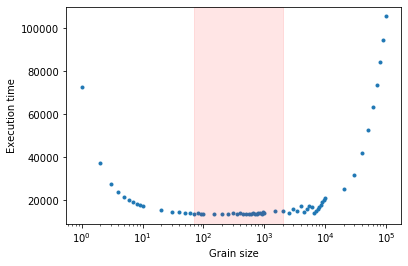
\includegraphics[scale=.42]{images/hpx_for_loop/marvin_100000_8.png}\label{fig60:a}}
	\subfloat[]
	{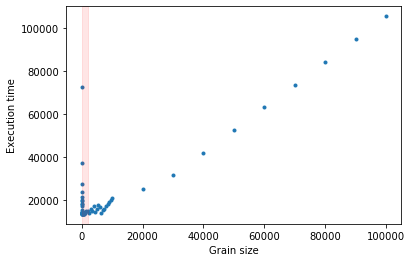
\includegraphics[scale=.42]{images/hpx_for_loop/marvin_100000_8nlog.png}\label{fig60:b}}
	\caption{The results of running the parallel for-loop benchmark with $problem\_size=100000$, on 8 cores. (a) represents the graph in logarithmic scale, while (b) shows the same graph in linear scale. The unit for execution time is microseconds.}\label{fig60}		
\end{figure}

Since our proposed model does not depend on the $problem\_{size}$ but relies on the number of tasks created, number of cores, and the time to execute the maximum amount of work assigned to a core, we are suggesting here that it might be sufficient to use the data collected from one $problem\_{size}$ to find the parameters $\alpha$ and $\sigma$. 
 
In order to test the viability of our proposition, we selected 5 different $problem\_{size}$s (10000, 100000, 1000000, 10000000, 100000000) to use as our base $problem\_{size}$ for finding the parameters of our model($\alpha$ and $\sigma$). 
Using all the collected data points for each \emph{problem\_{size}}, we utilized the \emph{optimize.curve\_{fit}} package from $scipy$ library in Python to fit our model to the collected data.

For any of the base \emph{problem\_{sizes}}, we measured the relative error and $R^2$ score of prediction for the base $problem\_{size}$ itself as shown in Formula~\ref{eq4} and Formula~\ref{eq5}. 
$p_i$ is the predicted value from curve fitting for sample $i$, $t_i$ is true value of that sample, and $n$ is the total number of samples.
The relative error and $R^2$ score are calculated for each specific number of cores individually. 

\begin{equation}{\label{eq4}}
Relative\_{error} = \frac{1}{n}\sum_{i=1}^{n} {|1-\frac{p_i}{t_i}|}
\end{equation}


\begin{equation}{\label{eq5}}
R^2 = 1-\frac{{\frac{1}{n}\sum_{i=1}^{n}{(t_i-p_i)}^2}}{Var(t)}
\end{equation}

Figure~\ref{fig59} illustrates the calculated relative error and $R^2$ score for \emph{problem\_{size}=10000, 100000, 1000000, 1000000, 100000000}. For each of the $problem\_{size}$s, 440, 512, 440, 512, and 728 data points were collected respectively. 

As the $problem\_{size}$ increases, we need to collect more data points to cover different regions of the grain size,  which results in longer total execution time of the benchmark. In order to rule out the uncertainties in our experiment as much as possible, we run each benchmark 6 times and take the average of the measured execution times. This means even larger overall execution time for data collection for larger $problem\_{sizes}$. 


\vspace{\baselineskip}
\begin{figure}[H]
	\centering
	\subfloat[]
	{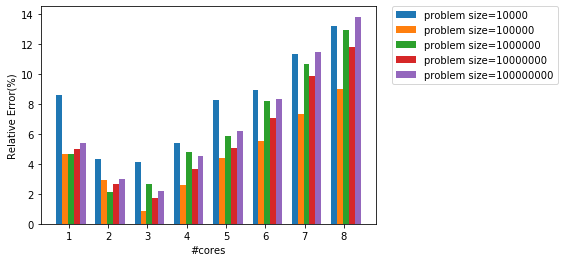
\includegraphics[scale=.45]{images/hpx_for_loop/fitted/marvin_relative_error_compared_self.png}}\label{fig59:a}
		\subfloat[]
	{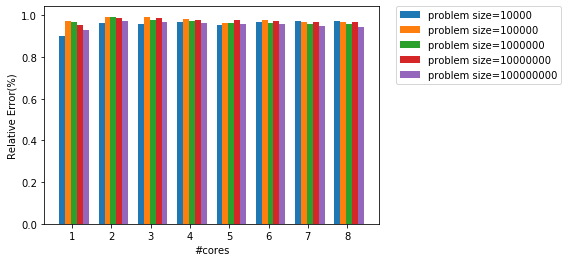
\includegraphics[scale=.45]{images/hpx_for_loop/fitted/marvin_r2_error_compared_self.png}}\label{fig59:b}
	\caption{The (a) relative error, and (b) $R^2$ score of fitting the collected data to the proposed analytical model for different $problem\_{sizes}$, calculated for each number of cores.}\label{fig59}		
\end{figure}

Figure~\ref{fig59} shows that for each number of cores, the calculated errors for each $problem\_{size}$ are very close to each other, and the the least amount of relative error was obtained when $problem\_{size}=100000$, which is most likely due to higher amount of data collected for this specific $problem\_{size}$. 

In the next step we measured the relative error and $R^2$ score of using the model parameters found from each base $problem\_{size}$ to predict the execution time for all other $problem\_{sizes}$. The result is illustrated in Figure~\ref{fig61}.
 
\vspace{\baselineskip}
\begin{figure}[H]
	\centering
	\subfloat[]
	{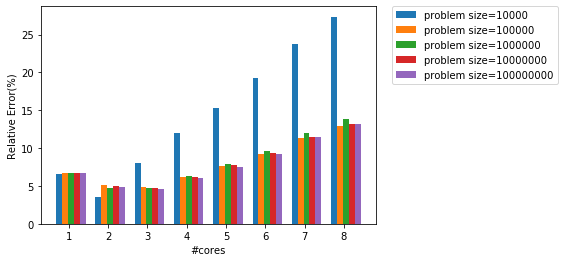
\includegraphics[scale=.45]{images/hpx_for_loop/fitted/marvin_relative_error_compared_rest.png}}\label{fig61:a}
	\subfloat[]
	{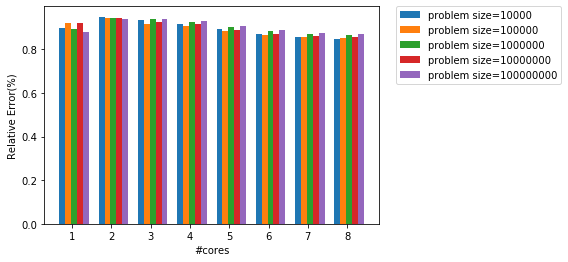
\includegraphics[scale=.45]{images/hpx_for_loop/fitted/marvin_r2_error_compared_rest.png}}\label{fig61:b}
	\caption{The (a)relative error and (b)$R^2$ score of using the model parameters found from each base $problem\_{size}$ fitting the proposed analytical model to the collected data for different $problem\_{sizes}$, calculated over each number of cores.}\label{fig61}		
\end{figure}

Based on Figure~\ref{fig60} and Figure\ref{fig61}, we selected $problem\_{size}=100000$ as the base\emph{problem\_{size}}, since it shows similar prediction error and $R^2$ score as larger $problem\_{size}s$, while taking less time to complete.

Having selected $problem\_{size}=100000$ as a reasonable(not too small nor too large) base for our parameter estimation, Figure~\ref{fig42} shows the measured execution time in terms of grain size for $problem\_{size}=100000$, with $N=1,2,...,8$.
 
 
\begin{figure}[H]
	\centering
	{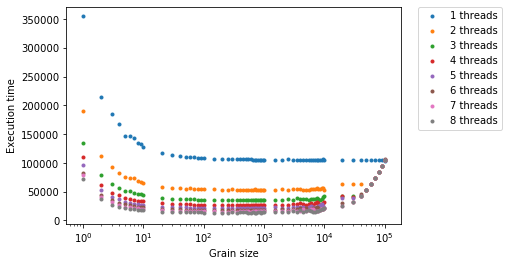
\includegraphics[scale=.7]{images/hpx_for_loop/marvin_100000_all.png}}
	\caption{The results of running the parallel for-loop benchmark with $problem\_size=100000$, on different number of cores. The unit for execution time is microseconds.}\label{fig42}		
\end{figure}
\vspace{\baselineskip}

Fitting our model to all the $512$ data points collected resulted in model parameters $alpha=2.674$ and $\sigma=0.0268$, where $\alpha$ represents the overhead of creating and managing the tasks in $\mu{secs}$, while $\sigma$ represents the contention based on Universal Scalibility Law.

\begin{figure}[H]
	\centering
	\subfloat[]
	{\centering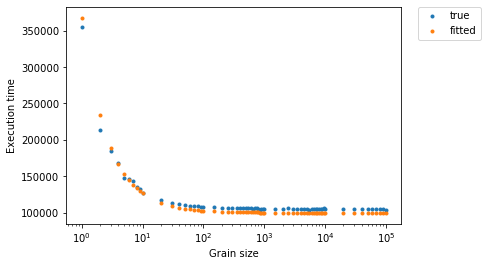
\includegraphics[scale=.35]{images/hpx_for_loop/fitted/100000/marvin_100000_1_100000.png}	
		\label{fig43:a}}
	\subfloat[]
	{\centering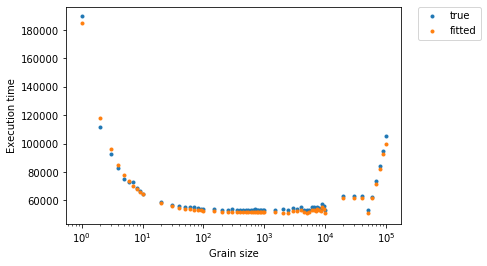
\includegraphics[scale=.35]{images/hpx_for_loop/fitted/100000/marvin_100000_2_100000.png}	
	\label{fig43:b}}\hfill
	\subfloat[]
	{\centering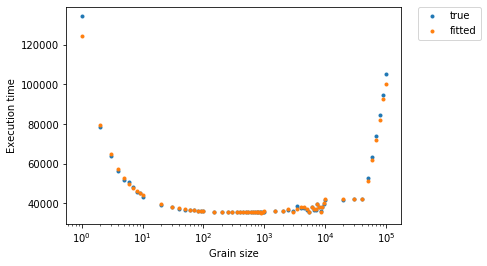
\includegraphics[scale=.35]{images/hpx_for_loop/fitted/100000/marvin_100000_3_100000.png}	
	\label{fig43:c}}
	\subfloat[]
	{\centering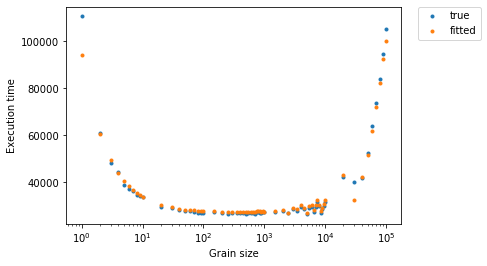
\includegraphics[scale=.35]{images/hpx_for_loop/fitted/100000/marvin_100000_4_100000.png}	
	\label{fig43:d}}\hfill
	\subfloat[]
	{\centering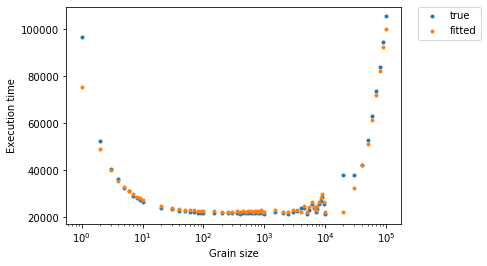
\includegraphics[scale=.35]{images/hpx_for_loop/fitted/100000/marvin_100000_5_100000.png}	
	\label{fig43:e}}
	\subfloat[]
	{\centering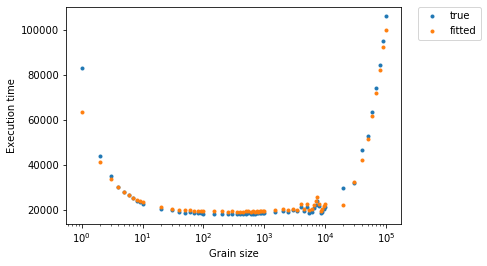
\includegraphics[scale=.35]{images/hpx_for_loop/fitted/100000/marvin_100000_6_100000.png}	
	\label{fig43:f}}\hfill
	\subfloat[]
	{\centering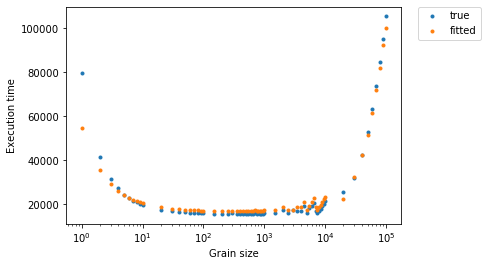
\includegraphics[scale=.35]{images/hpx_for_loop/fitted/100000/marvin_100000_7_100000.png}	
		\label{fig43:g}}
	\subfloat[]
	{\centering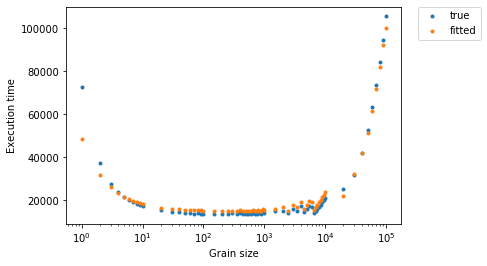
\includegraphics[scale=.35]{images/hpx_for_loop/fitted/100000/marvin_100000_8_100000.png}	
	\label{fig43:h}}\hfill
	\caption{The results of predicted values of execution time through curve fitting vs the real data for $problem\_size=100000$, for (a) 1 core, (b) 2 cores, (c) 3 cores, (d) 4 cores, (e) 5 cores, (f) 6 cores, (g) 7 cores, (h) 8 cores. The unit for execution time is microseconds.}
	\label{fig43}	
\end{figure}

Figure~\ref{fig43} shows the fitted curves along with the original data for different number of cores.


\begin{figure}[H]
	\centering
	\subfloat[]
	{\centering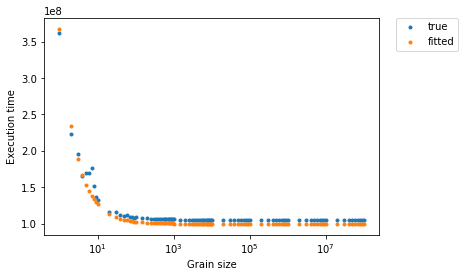
\includegraphics[scale=.35]{images/hpx_for_loop/fitted/100000/marvin_100000000_1_100000.png}	
		\label{fig62:a}}
	\subfloat[]
	{\centering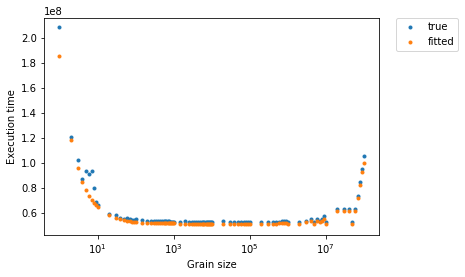
\includegraphics[scale=.35]{images/hpx_for_loop/fitted/100000/marvin_100000000_2_100000.png}	
		\label{fig62:b}}\hfill
	\subfloat[]
	{\centering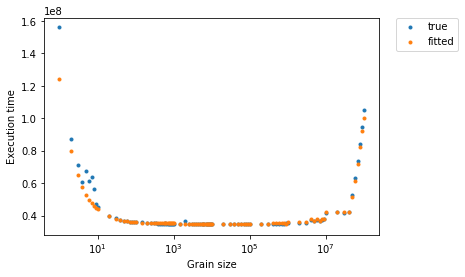
\includegraphics[scale=.35]{images/hpx_for_loop/fitted/100000/marvin_100000000_3_100000.png}	
		\label{fig62:c}}
	\subfloat[]
	{\centering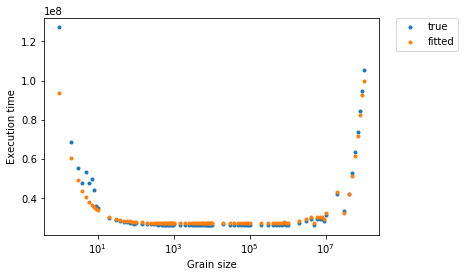
\includegraphics[scale=.35]{images/hpx_for_loop/fitted/100000/marvin_100000000_4_100000.png}	
		\label{fig62:d}}\hfill
	\subfloat[]
	{\centering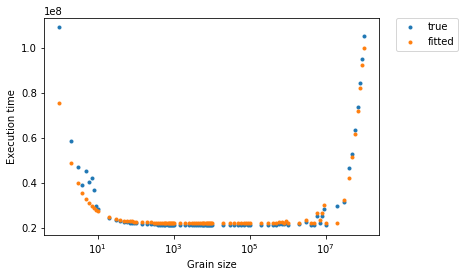
\includegraphics[scale=.35]{images/hpx_for_loop/fitted/100000/marvin_100000000_5_100000.png}	
		\label{fig62:e}}
	\subfloat[]
	{\centering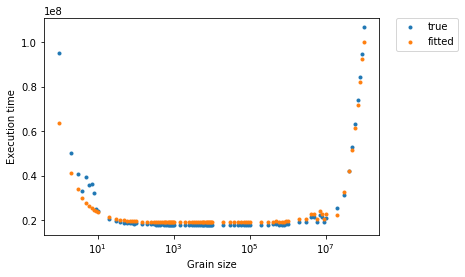
\includegraphics[scale=.35]{images/hpx_for_loop/fitted/100000/marvin_100000000_6_100000.png}	
		\label{fig62:f}}\hfill
	\subfloat[]
	{\centering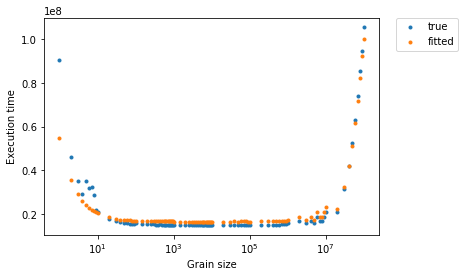
\includegraphics[scale=.35]{images/hpx_for_loop/fitted/100000/marvin_100000000_7_100000.png}	
		\label{fig62:g}}
	\subfloat[]
	{\centering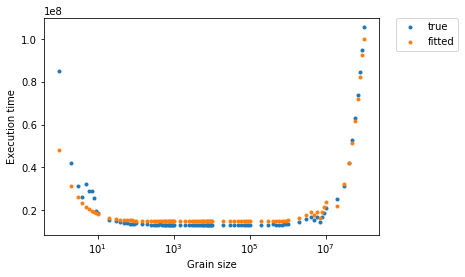
\includegraphics[scale=.35]{images/hpx_for_loop/fitted/100000/marvin_100000000_8_100000.png}	
		\label{fig62:h}}\hfill
	\caption{The results of predicted values of execution time through curve fitting vs the real data for $problem\_size=100000000$, for (a) 1 core, (b) 2 cores, (c) 3 cores, (d) 4 cores, (e) 5 cores, (f) 6 cores, (g) 7 cores, (h) 8 cores. The unit for execution time is microseconds.}
	\label{fig62}	
\end{figure}


\subsection{Testing the Proposed Model on Other Architectures}

At the next step we repeated the same process for the data collected from two different architectures, \textit{Medusa} node with a Skylake CPU, and a Raspberry Pi 4.

\subsection{Medusa}
We used $problem\_{size}=100000$ as the base \emph{problem\_{size}} on both architectures. On Medusa, with $problem\_{size}=100000$, the model parameters were found to be $\alpha=1.832$ and $\sigma=0.037$. 
The calculated relative error and $R^2$ score for each individual number of cores for $problem\_{size}=100000$ is demonstrated in Figure~\ref{fig64}, and Figure~\ref{fig63}, while the relative error and $R^2$ score calculated for all other \emph{problem\_{sizes}} is shown in Figure~\ref{fig64}, and Figure~\ref{fig63}.
\vspace{\baselineskip}

\begin{figure}[H]
	\centering
	\subfloat[]
	{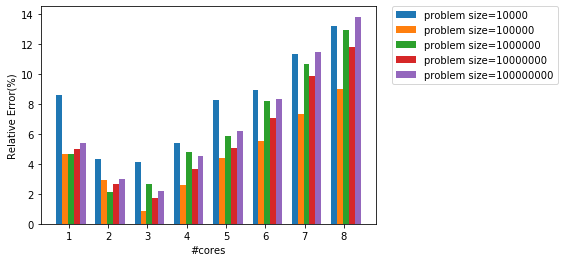
\includegraphics[scale=.45]{images/hpx_for_loop/fitted/marvin_relative_error_compared_self.png}}\label{fig64:a}
	\subfloat[]
	{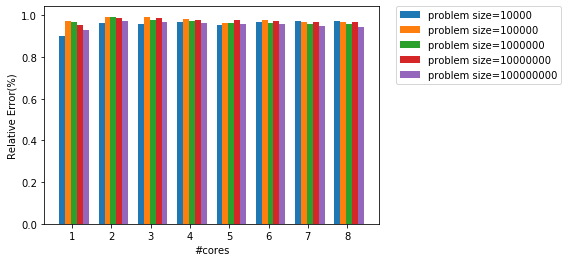
\includegraphics[scale=.45]{images/hpx_for_loop/fitted/marvin_r2_error_compared_self.png}}\label{fig64:b}
	\caption{The (a) relative error, and (b) $R^2$ score of fitting the collected data to the proposed analytical model for different $problem\_{sizes}$, calculated for each number of cores.}\label{fig64}		
\end{figure}

\vspace{\baselineskip}
\begin{figure}[H]
	\centering
	\subfloat[]
	{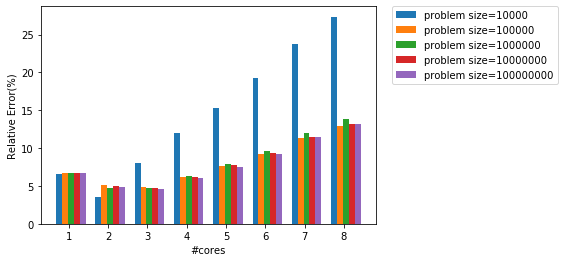
\includegraphics[scale=.45]{images/hpx_for_loop/fitted/marvin_relative_error_compared_rest.png}}\label{fig63:a}
	\subfloat[]
	{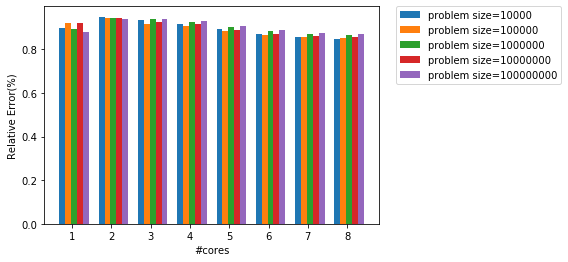
\includegraphics[scale=.45]{images/hpx_for_loop/fitted/marvin_r2_error_compared_rest.png}}\label{fig63:b}
	\caption{The (a)relative error and (b)$R^2$ score of using the model parameters found from each base $problem\_{size}$ fitting the proposed analytical model to the collected data for different $problem\_{sizes}$, calculated over each number of cores.}\label{fig63}
\end{figure}

\begin{figure}[H]
	\centering
	\subfloat[]
	{\centering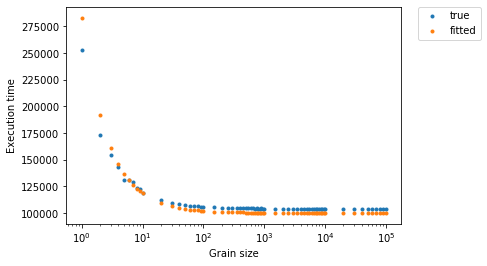
\includegraphics[scale=.4]{images/hpx_for_loop/fitted/100000/medusa_100000_1_100000.png}	
		\label{fig50:a}}
	\subfloat[]
	{\centering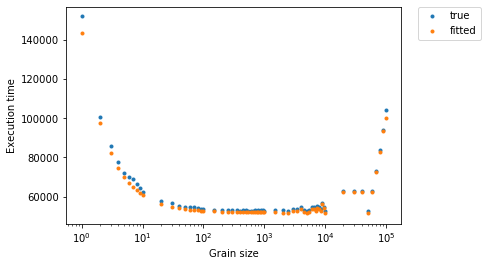
\includegraphics[scale=.4]{images/hpx_for_loop/fitted/100000/medusa_100000_2_100000.png}	
		\label{fig50:b}}\hfill
	\subfloat[]
	{\centering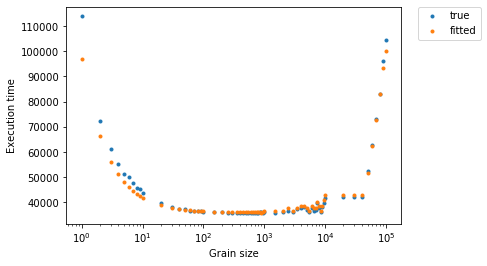
\includegraphics[scale=.4]{images/hpx_for_loop/fitted/100000/medusa_100000_3_100000.png}	
		\label{fig50:c}}
	\subfloat[]
	{\centering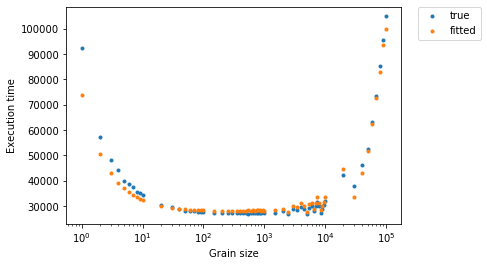
\includegraphics[scale=.4]{images/hpx_for_loop/fitted/100000/medusa_100000_4_100000.png}	
		\label{fig50:d}}\hfill
	\subfloat[]
	{\centering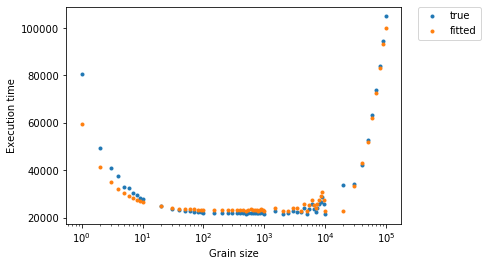
\includegraphics[scale=.4]{images/hpx_for_loop/fitted/100000/medusa_100000_5_100000.png}	
		\label{fig50:e}}
	\subfloat[]
	{\centering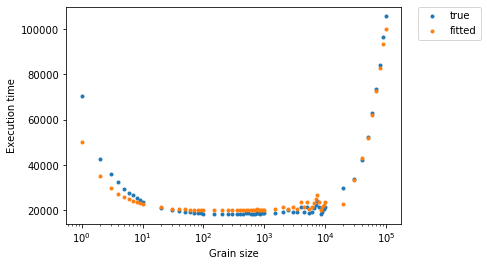
\includegraphics[scale=.4]{images/hpx_for_loop/fitted/100000/medusa_100000_6_100000.png}	
		\label{fig50:f}}\hfill
	\subfloat[]
	{\centering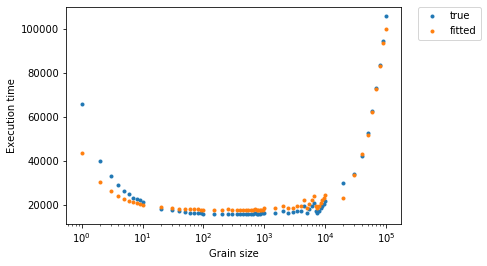
\includegraphics[scale=.4]{images/hpx_for_loop/fitted/100000/medusa_100000_7_100000.png}	
		\label{fig50:g}}
	\subfloat[]
	{\centering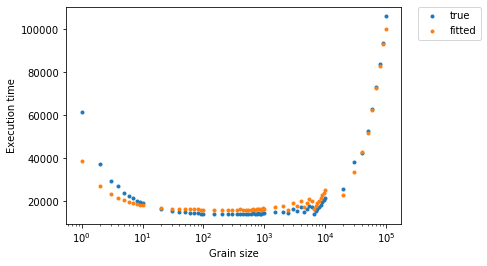
\includegraphics[scale=.4]{images/hpx_for_loop/fitted/100000/medusa_100000_8_100000.png}	
		\label{fig50:h}}\hfill
	\caption{The results of predicted values of execution time through curve fitting vs the real data for $problem\_size=100000$, for (a) 1 core, (b) 2 cores, (c) 3 cores, (d) 4 cores, (e) 5 cores, (f) 6 cores, (g) 7 cores, (h) 8 cores. The unit for execution time is microseconds.}
	\label{fig50}	
\end{figure}

\subsection{Raspberry Pi 4}


\vspace{\baselineskip}
\subsection{Analyzing the Data}
Assuming the proposed formula is a good fit for this problem, we can estimate the range of grain sizes for which we achieve the lowest execution time, for a specific problem size, ran on specific number of cores.

\vspace{\baselineskip}
\subsubsection{Left side of the Graph}
As stated earlier, in Formula~\ref{formula1}, for small grain sizes the first term is the dominant factor while the second term roughly stays constant. Same way, for large grain sizes the second factor is the dominant factor. 

In order to find the lower-bound of the range for which the execution time stays constant, we assume the second factor is constant in that region. Also we can change $N$ to $M$, knowing that our concern is on the left hand side of the graph, where $num\_{tasks}$ is definitely greater than the number of cores. 
Taking the derivative of the function based on the grain size then leads to:

 
\begin{equation}\label{formula3}
\begin{aligned}
\frac{\partial execution\_{time}}{\partial g} &= \frac{\alpha}{N}\times{\frac{\partial num\_{tasks}}{\partial g}}\\
&=\frac{\alpha}{N}\times\frac{\partial(\frac{problem\_{size}}{g})}{\partial g} \\
&=\frac{\alpha}{N}\times{problem\_{size}}\times{\frac{-1}{g^2}}
\end{aligned}
\end{equation}

From Formula~\ref{formula3}, it can be observed that for the left hand side of the graph the rate of changes is negative and decreases as the grain size increases. Here we are looking for the value of the grain size for which the rate of change becomes very small (we introduce a threshold $\lambda_b$, where $\lambda_b\ll1$, for this purpose). 


\begin{equation}\label{formula4}
\begin{aligned}
&\frac{\alpha}{N}\times{problem\_{size}}\times{\frac{1}{g^2}}\leq{\lambda_b} \\
{g^2}&\geq{\frac{\frac{\alpha}{N}\times{problem\_{size}}}{\lambda_b}}\\
{g}&\geq{\sqrt{\frac{\frac{\alpha}{N}\times{problem\_{size}}}{\lambda_b}}}
\end{aligned}
\end{equation}

Formula~\ref{formula4} can also be represented as shown in Formula~\ref{formula5}. This representation shows that when the ratio of the time it takes to execute one task to the total overhead of creating and managing $num\_{tasks}$ tasks on $N$ core, is greater than a threshold, we will end up in the flat region of the graph, close to the left hand side.


\begin{equation}\label{formula5}
\begin{aligned}
\frac{\alpha}{N}\times{\frac{problem\_{size}}{g}}\times{\frac{1}{g}}&\leq{\lambda_b}\\
\frac{\alpha}{N}\times{num\_{tasks}}\times{\frac{1}{g}}&\leq{\lambda_b}\\
\frac{\alpha}{N}\times{num\_{tasks}}&\leq{g\times\lambda_b}\\	
\frac{g}{\frac{\alpha}{N}\times{num\_{tasks}}}&\geq{\frac{1}{\lambda_b}}
\end{aligned}
\end{equation}


\subsubsection{Right side of the graph}
Now looking at the right hand side of the graph, the overhead of creating the tasks becomes negligible on that side, since only few tasks are being created and the overhead of creating these many tasks is not significant compared to the execution time. On this side, the maximum amount of work executed by one core ($w\_c$) and consequently the time to perform this amount of work ($t\_c$) is the dominant factor.

Formula~\ref{formula2} shows how $w\_c$ is calculated for different cases, but in general we can estimate $w\_c$ with $g\times\left \lceil{\frac{num\_{tasks}}{N}}\right \rceil$. 

\begin{equation}\label{formula6}
\begin{aligned}
w\_c&\approx{g\times\left \lceil{\frac{num\_{tasks}}{N}}\right \rceil}\\
&\approx{g\times\left \lceil{\frac{\frac{problem\_{size}}{g}}{N}}\right \rceil}\\
&\approx{\frac{problem\_{size}}{N}} \:\:\text{\:\:\:\:if\:\:} num\_{tasks}\geq{N}
\end{aligned}
\end{equation}

What happens here is that as the grain size changes, there are points for which $\left \lceil{\frac{num\_{tasks}}{N}}\right \rceil$ is the same but since the grain size is different, a different $w\_c$ would be resulted. 
For all the values of $g$ that create the same $\left \lceil{\frac{num\_{tasks}}{N}}\right \rceil$, as $g$ increases the difference between $w\_c$ and $\frac{problem\_{size}}{N}$ increases. 

For example, considering a case where $problem\_{size}=100,000$, and $N=8$, for the grain sizes in range of $[4167,\:6249]$ would result in creating between $\left \lceil{\frac{100,000}{6,249}}\right \rceil=17$ and  $\left \lceil{\frac{100,000}{4,167}}\right \rceil=24$ tasks. This amount of tasks created itself would result in $\left \lceil{\frac{17}{8}}\right \rceil=3$ and  $\left \lceil{\frac{24}{8}}\right \rceil=3$ tasks.
On the other hand, $w\_c=g\times{\left \lceil{\frac{num\_{tasks}}{N}}\right \rceil}=3\times{g}$, would have a value in range of $[3\times4167,\:3\times6249]=[12501,\: 18747]$, where the average amount of work per core is $\frac{problem\_{size}}{N}=12500$. This means that for grain sizes closer to the end of the range, we are observing that a much bigger amount of work is assigned to the core with maximum amount of work, which would result in a higher execution time. 


In the general case, if we denote $\left \lceil{\frac{num\_{tasks}}{N}}\right \rceil$ as $k$, then:


\begin{equation}\label{formula8}
\begin{aligned}
k-1&<{\frac{num\_{tasks}}{N}}\leq{k}\\
(k-1)\times{N}&<num\_{tasks}\leq{k}\times{N}\\
%num\_{tasks}=\left \lceil{\frac{problem\_{size}}{g}}\right \rceil\\
(k-1)\times{N}&<\left \lceil{\frac{problem\_{size}}{g}}\right \rceil\leq{k}\times{N}\\
(k-1)\times{N}&<\frac{problem\_{size}}{g}\leq{{k}\times{N}}\\
\end{aligned}
\end{equation}

If $k=1$, then, 

\begin{equation}\label{formula9}
\begin{aligned}
0<\frac{problem\_{size}}{g}\leq{N}\\
\frac{problem\_{size}}{N}\leq{g}\leq{problem\_{size}}.
\end{aligned}
\end{equation}

Otherwise, when $k>1$,

\begin{equation}\label{formula10}
\begin{aligned}
\frac{problem\_{size}}{k\times{N}}\leq{g}<\frac{problem\_{size}}{(k-1)\times{N}}.
\end{aligned}
\end{equation}

Since $\left \lceil{\frac{num\_{tasks}}{N}}\right \rceil=k$, and $w\_c={g\times\left \lceil{\frac{num\_{tasks}}{N}}\right \rceil}={k\times{g}}$ if $num\_{tasks}\%{N}\neq{1}$, we can conclude for $k>1$:

\begin{equation}\label{formula11}
\begin{aligned}
k\times{\frac{problem\_{size}}{k\times{N}}}&\leq{w\_c}<{k\times{\frac{problem\_{size}}{(k-1)\times{N}}}}\\
\frac{problem\_{size}}{{N}}&\leq{w\_c}<{\frac{k}{k-1}\times{\frac{problem\_{size}}{N}}}\\
0&\leq{w\_c-\frac{problem\_{size}}{N}}<\frac{1}{k-1}\times{\frac{problem\_{size}}{N}}
\end{aligned}
\end{equation}

For the cases where $k>1$ and $num\_{tasks}\%{N}={1}$, there could be a  change in $w\_c$ if $problem\_{size}\%{g}\neq{0}$. For these cases:


\begin{equation}\label{formula15}
\begin{aligned}
\left \lceil{\frac{num\_{tasks}}{N}}\right \rceil&=k \text{\:\:\:}\&\text{\:\:\:} num\_{tasks}\%{N}={1}\Rightarrow\\
num\_{tasks}&=(k-1)\times{N}+1\Rightarrow\\
(k-1)\times{N}&<{\frac{problem\_{size}}{g}}\leq(k-1)\times{N}+1\Rightarrow\\
\frac{problem\_{size}}{(k-1)\times{N}+1}&\leq{g}<\frac{problem\_{size}}{(k-1)\times{N}}
\end{aligned}
\end{equation}

From Formula~\ref{formula2} we know,
\begin{equation}\label{formula17}
\begin{aligned}
w\_c={problem\_{size}}-(k-1)\times(N-1)\times{g}.
\end{aligned}
\end{equation}

Therefore,
\begin{equation}\label{formula18}
\begin{aligned}
(k-1)(N-1)\frac{problem\_{size}}{(k-1){N}+1}&\leq{(k-1)(N-1){g}}<(k-1)(N-1)\frac{problem\_{size}}{(k-1){N}}\Rightarrow\\
{\frac{problem\_{size}}{N}}&<{problem\_{size}-{(k-1)(N-1){g}}}\leq{k\frac{problem\_{size}}{(k-1){N}+1}}\\
{\frac{problem\_{size}}{N}}&<{w\_{c}}\leq{k\times\frac{problem\_{size}}{(k-1){N}+1}}
\end{aligned}
\end{equation}

And for $k=1$, where $num\_{tasks}\leq{N}$,
\begin{align*}\label{formula12}
w\_c&=g\\
\frac{problem\_{size}}{N}&\leq{g}\leq{problem\_{size}}\Rightarrow
\end{align*}

\begin{equation}\label{formula14}
\begin{aligned}
0\leq{w\_c-\frac{problem\_{size}}{N}}={g-\frac{problem\_{size}}{N}}\leq(N-1)\times{\frac{problem\_{size}}{N}}\\
\end{aligned}
\end{equation}


Defining $imbalance\_{ratio}=\frac{w\_c-\frac{problem\_{size}}{N}}{\frac{problem\_{size}}{N}}$, then,

\begin{equation}\label{formula13}
\begin{aligned}
0&\leq{imbalance\_{ratio}}\leq{N-1}  \text{\:\:\:\:\:\:\:\:\:\:\:\:\:for\:\:\:}k={1}\\
0&\leq{imbalance\_{ratio}}<\frac{1}{k-1}  \text{\:\:\:\:\:\:\:\:\:\:\:\:\:for\:\:\:}k>{1} \text{\:\:and\:\:}num\_{tasks}\%{N}\neq{1}\\
0&\leq{imbalance\_{ratio}}<\frac{N-1}{N(k-1)+1}=\frac{1}{k-1+\frac{k}{N-1}}\text{\:\:\:\:\:\:\:\:\:\:\:\:\:otherwise}
\end{aligned}
\end{equation}

%k\in\mathbb{Z}
Formula~\ref{formula13} shows that as number of created tasks increases, as long as number of tasks per core is the same, the imbalance factor decreases. 

\vspace{\baselineskip}

Figure~\ref{fig38} shows the imbalance ratio calculated for different grain sizes for $problem\_size=10000$, on 8 cores. Each of the regions between two dashed green lines correspond to a specific value for $k=\left\lceil{\frac{num\_{tasks}}{N}}\right \rceil$. 
At each of the regions with $k>1$, $\left\lceil{\frac{num\_{tasks}}{N}}\right \rceil=k$,  $imbalance\_{ratio}$ starts from $0$ and approaches $\frac{1}{k-1}$ ($\frac{1}{k-1+\frac{k}{N-1}}$ for regions where $num\_{tasks}\%{N}\neq{1}$) at the end of the region. When $k=1$, $imbalance\_{ratio}$ increases linearly starting from 0 and reaching the maximum of $N-1$ when $g=pronblem\_{size}$. As we move to larger grain sizes, $\left\lceil{\frac{num\_{tasks}}{N}}\right \rceil$ decreases, therefore the upper-bound for $imbalance\_{ratio}$ increases.   


\vspace{\baselineskip}	
\begin{figure}[H]
	\centering
	{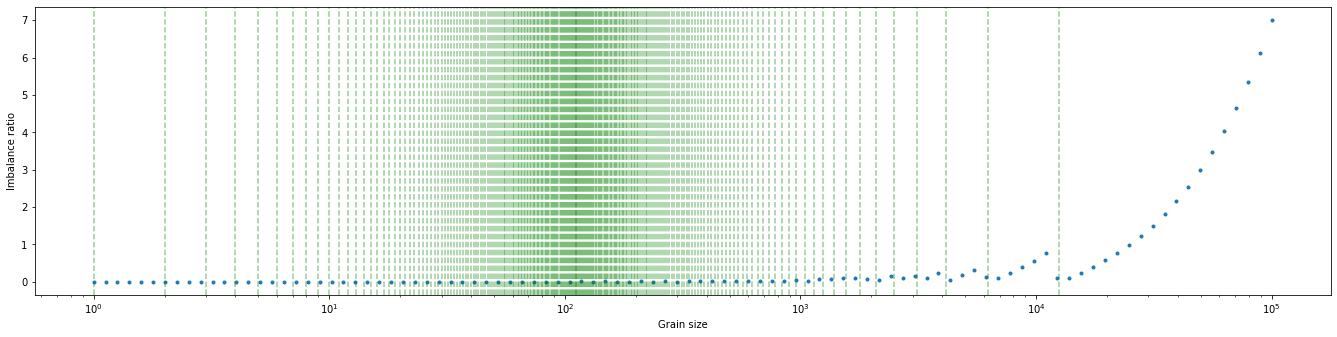
\includegraphics[scale=.25]{images/hpx_for_loop/imbalance_ratio_100000_8.png}}
	\caption{The imbalance ratio calculated for different grain sizes for $problem\_size=10000$, on 8 cores. At the area between each two green lines $k=\left\lceil{\frac{num\_{tasks}}{N}}\right \rceil$ is constant.}\label{fig38}		
\end{figure}


%\vspace{\baselineskip}	
%\begin{figure}[H]
%	\centering
%	{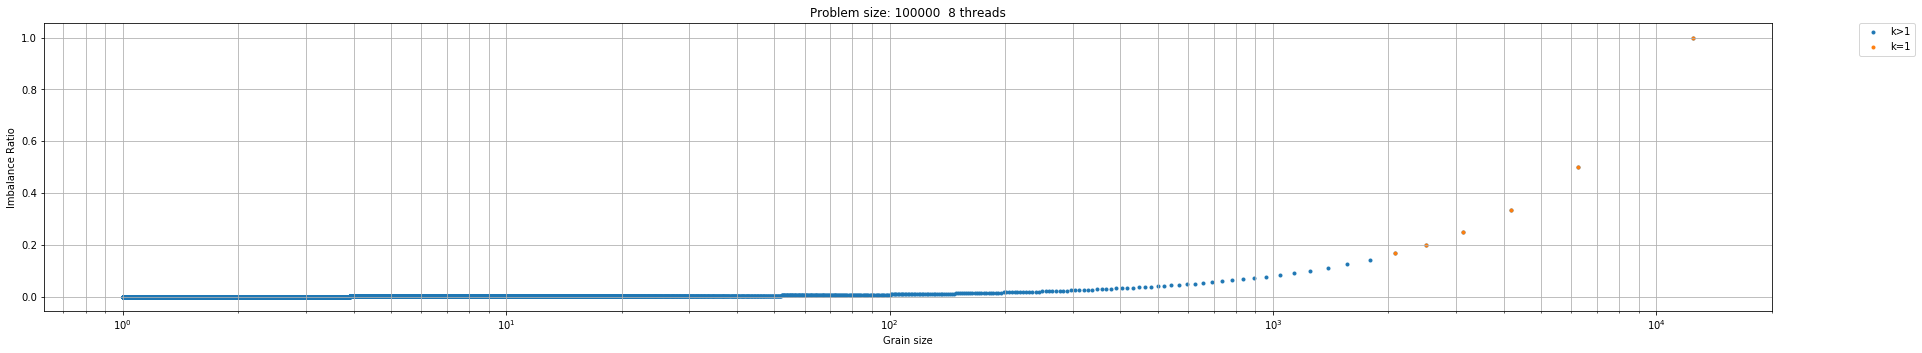
\includegraphics[scale=.45]{images/hpx_for_loop/max_w_c.png}}
%	\caption{The maximum imbalance ratio calculated for different grain sizes for $problem\_size=10000$, on 8 cores, where $k=\left\lceil{\frac{num\_{tasks}}{N}}\right \rceil$.}\label{fig36}		
%\end{figure}

Figure~\ref{fig37} represents the imbalance ratio, along with the ratio of the sequential execution time over execution time(speed-up) against grain size for $problem\_size=10000$, ran on 8 cores.   
As it can be observed, as the $imbalance\_{ratio}$ increases, the speed-up decreases. 

\vspace{\baselineskip}	
\begin{figure}[H]
	\centering
	{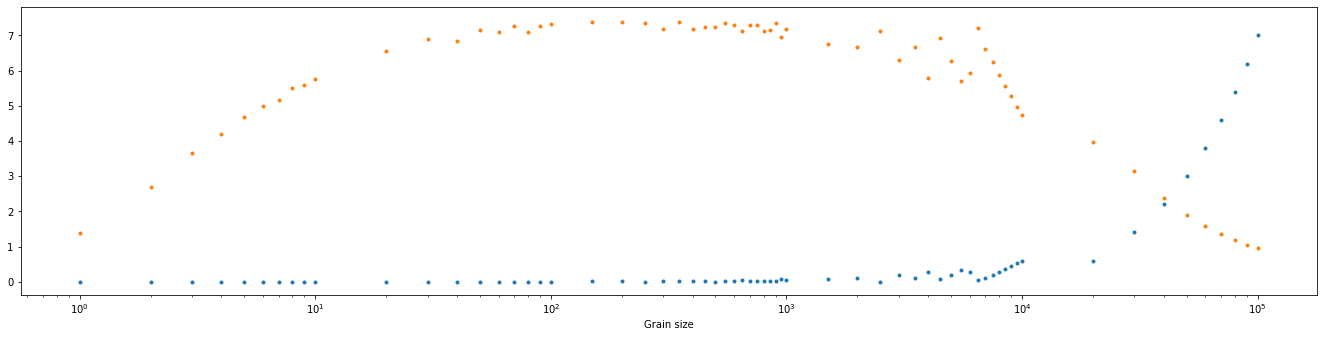
\includegraphics[scale=.3]{images/hpx_for_loop/imbalance_ratio_speedup_100000_8.png}}
	\caption{The imbalance ratio alongside speedup for different grain sizes for $problem\_size=10000$, on 8 cores, where $k=\left\lceil{\frac{num\_{tasks}}{N}}\right \rceil$.}\label{fig37}		
\end{figure}


To summarize, as the grain size increases the maximum imbalance in the loads assigned to the cores also increases, and some point on, this imbalance has a significant affect in the execution time. We define a threshold, $\lambda_s$ ($0<\lambda_s<1$), where for $imbalance\_{ratio}$s smaller than this threshold the imbalance effect is not significant. As we get close to this threshold, we are likely to reach the right hand side of the flat region of the bathtub curve of the execution time against grain size. 


We are interested in finding the maximum grain size that would generate a reasonable imbalance ($imbalance\_{ratio}\leq{\lambda_s}$), to make sure we should stay in the flat region of the bathtub curve of execution time against grain size, from load imbalance point of view.  

Formula~\ref{formula14} states that for grain sizes greater than $problem\_{size}$, $imblance\_{ratio}$ increases linearly with grain size from $0$ to $N-1$. While for grain sizes smaller than $problem\_{size}$, the maximum $imbalance\_{ratio}$ depends on $k=\left\lceil{\frac{num\_{tasks}}{N}}\right\rceil$. So, in order to ensure \emph{imbalance\_{ratio}} is smaller than or equal to a threshold ($\lambda_s$), first we search the grain sizes smaller than $\frac{problem\_{size}}{N}$. Since $0<\lambda_s<1$, and $k\geq2$ in this region, there exists a $k$ such that $\frac{1}{k-1}\leq\lambda_s$.    
If there exists a $k_{min}$ (creating an imbalance ratio between $0$ and $\frac{1}{k_{min}-1}$), where $\frac{1}{k_{min}-1}\leq{\lambda_s}$, $\forall k<k_{min}$ maximum value of $imbalance\_{ratio}$ would be greater than $\lambda_s$. So in order to find the grain size that would create maximum $imbalance\_{ratio}$ of $\lambda_s$:



\begin{equation}\label{formula21}
\begin{aligned}
&imbalance\_{ratio}\leq{{\lambda_s}}\Rightarrow\\
&\frac{1}{k-1}\leq\lambda_s\\
&k\geq{1+\frac{1}{\lambda_s}}\\
&k_{min}=\left\lceil{1+\frac{1}{\lambda_s}}\right\rceil+1\\
&{g}<\frac{problem\_{size}}{(k_{min}-1)\times{N}}\\
&g_{max}=\frac{problem\_{size}}{(k_{min}-1)\times{N}}-1=\frac{problem\_{size}}{(1+\left\lceil{\frac{1}{\lambda_s}}\right\rceil)\times{N}}
\end{aligned}
\end{equation}

If $g<g\_{max}$, we can ensure that $imbalance\_{ratio}$ never exceeds $\lambda_s$. Since we already found a match at grain sizes smaller than $\frac{problem\_{size}}{N}$, checking the rest of grain sizes would not be necessary.



\vspace{\baselineskip}
\subsection{Identifying the Range of Grain Size for Minimum Execution Time}
In the previous section, we proposed a method to identify the lower-bound and the upper-bound of the grain sizes for which we expect to observe the minimum execution time. 
Integrating Formula~\ref{formula4} and Formula~\ref{formula21} suggests the following range for minimum execution time:


\begin{equation}\label{formula23}
\begin{aligned}
{\sqrt{\frac{(\frac{\alpha}{N})\times{problem\_{size}}}{{\lambda_b}}}}\leq{g}\leq\frac{problem\_{size}}{(1+\left\lceil{\frac{1}{\lambda_s}}\right\rceil)\times{N}}
\end{aligned}
\end{equation}
 
Where $0\leq\lambda_s\leq1$, and $\lambda_b,\lambda_s\ll1$.

Note that based on Formula~\ref{formula23} we can state,

\begin{equation}\label{formula43}
\begin{aligned}
{\sqrt{\frac{(\frac{\alpha}{N})\times{problem\_{size}}}{{\lambda_b}}}}\leq{g}\leq\frac{problem\_{size}}{(1+\left\lceil{\frac{1}{\lambda_s}}\right\rceil)\times{N}}<\frac{problem\_{size}}{N}.
\end{aligned}
\end{equation}

Which shows that the identified range of minimum execution time is located at the left side of the grain size that equally divides the work between the cores, $\frac{problem\_{size}}{N}$.
  
\vspace{\baselineskip}
\subsection{Locating the Flat Region of the Execution time vs Grain Size Graph for the Benchmark}
In this section we used Formula~\ref{formula23} to identify the flat region of the execution time vs grain size graph for the parallel for-loop benchmark in Listing~\ref{hpx_for_loop}. For this purpose, we set  both $\lambda_{b}$ and $\lambda_{s}$ to $0.1$. The minimum and maximum acceptable value for grain size to lay in the flat region of the graph are then calculated based on Formula~\ref{formula43}. $\lambda_{b}$ indicates the slope of the graph at the left hand side of the graph where overhead of tasks is the dominant factor. $\lambda_{b}=0.1$ shows an angle of around $5\textdegree$, which seems to be a reasonable threshold. Grain sizes smaller than $\sqrt{\frac{(\frac{\alpha}{N})\times{problem\_{size}}}{{\lambda_b}}}$ would create a slope of more than $\lambda_b$. As for $\lambda_s$, a grain size greater than       
$\frac{problem\_{size}}{(1+\left\lceil{\frac{1}{\lambda_s}}\right\rceil)\times{N}}$ could generate an $imbalance\_{ratio}$ of greater than $\lambda_s$. Therefore, for grain sizes within the range in Formula~\ref{formula43} we are in a safe region. 
 
In Figure~\ref{fig51} the identified regions for minimum execution time is shown in green, for $problem\_{size}=10000,\:100000,\:1000000,\:10000000,\:100000000$, executed on $8$ cores. The gray dashed line represents the grain size where work is equally divided among the cores, $\frac{problem\_size}{N}$.

\begin{figure}[H]
	\centering
	\subfloat[]
	{\centering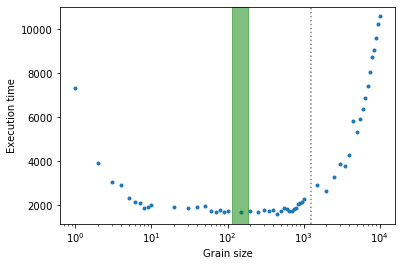
\includegraphics[scale=.4]{images/hpx_for_loop/fitted/100000/marvin_10000_8_range_10_10.png}	
		\label{fig51:a}}
	\subfloat[]
	{\centering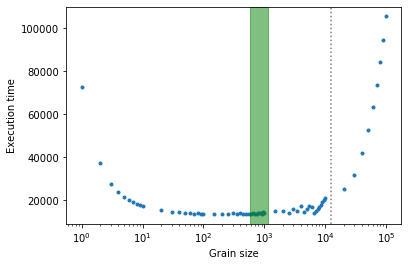
\includegraphics[scale=.4]{images/hpx_for_loop/fitted/100000/marvin_100000_8_range_10_10.png}	
		\label{fig51:b}}\hfill
	\subfloat[]
	{\centering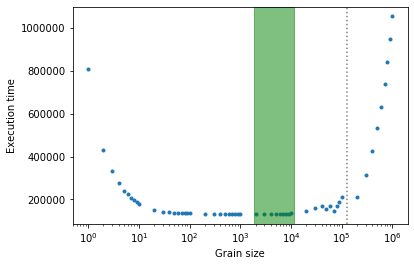
\includegraphics[scale=.4]{images/hpx_for_loop/fitted/100000/marvin_1000000_8_range_10_10.png}	
		\label{fig51:c}}
	\subfloat[]
	{\centering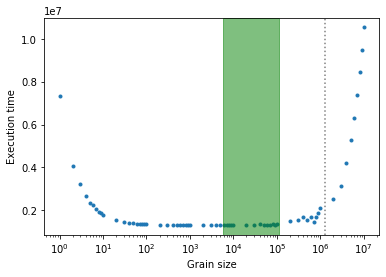
\includegraphics[scale=.4]{images/hpx_for_loop/fitted/100000/marvin_10000000_8_range_10_10.png}	
		\label{fig51:d}}\hfill
	\subfloat[]
	{\centering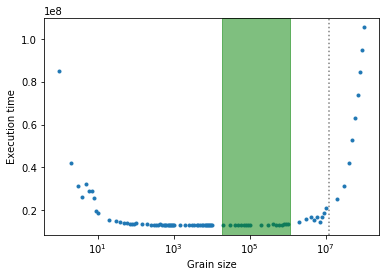
\includegraphics[scale=.4]{images/hpx_for_loop/fitted/100000/marvin_100000000_8_range_10_10.png}	
		\label{fig51:e}}
	\caption{The identified range of grain size for minimum execution time for $problem\_size=$ (a) 10000, (b) 100000, (c) 1000000, (d) 10000000, (e) 100000000, on 8 cores, with $\lambda_{s}=0.1$ and $\lambda_{b}=0.1$. The gray dashed line represents the grain size where work is equally divided among the cores, $\frac{problem\_size}{N}$. The unit for execution time is microseconds.}
	\label{fig51}	
\end{figure}

Selecting a greater value for $\lambda_b$ would move the left border of the region to left, for a larger acceptable slope of change of execution time in terms of grain size. On the other hand, selecting a smaller value for $\lambda_{s}$ would result in shifting the right border of the region to left, imposing a higher restriction on $imbalance\_{ratio}$, as shown in Figure~\ref{fig65}.

\vspace{\baselineskip}	
\begin{figure}[H]
	\centering
	{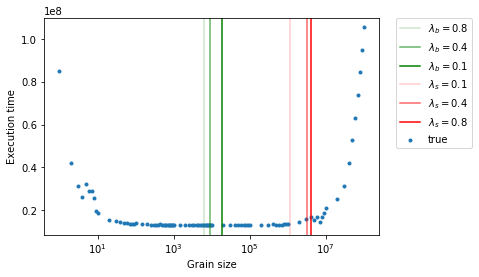
\includegraphics[scale=.6]{images/hpx_for_loop/fitted/100000/marvin_100000000_8_range_10_50_80.png}}
	\caption{An example of the effect of $\lambda_b$ and $\lambda_s$ on the borders of the identified region for minimum execution time due to change for $problem\_{size}=100000000$ and $N=8$. }\label{fig65}		
\end{figure}
    


\subsection{Applying the Proposed Model to the Blazemark Data}
In the previous section we proposed an analytical model to predict how execution time changes with grain size, and suggested a method to estimate the range of grain size for a specific $problem\_{size}$ ran on a certain number of cores to stay in the region of minimum execution time. We then tested the proposed model on a simple parallel for-loop benchmark, an the results seemed promising.
In this section we revisit our original problem of finding the range of chunk size for minimum execution time to calculate an expression using the Blaze linear algebra library. 
We start by looking at the data collected from $DMATDMATADD$ benchmark, which represents addition of two row major square dense matrices.
  
As we previously stated in Chapter~\ref{Method}, for the collected data, the \emph{DMATDMATADD} benchmark was executed with different configurations of $block\_{size}$, $chunk\_{size}$, and number of cores, for different matrix sizes. 
As discussed earlier the collected data suggested that instead of looking at $block\_{size}$ and then $chunk\_{size}$, we can study the effect of grain size on execution time. By identifying the range of grain size that ensures staying in the flat region of the bathtub, we can then select a reasonable value for $block\_{size}$, we can find the range of $chunk\_{sizes}$ to generate the mentioned range of grain size. We define a reasonable value for block size for an operation on row major matrices, az the size of a matrix with larger number of columns than number of rows, where number of columns is divisible by cache line, and the number of elements in the block multiplied by number of matrices involved in an operation, is smaller than L2 cache size. With these assumptions we selected the value of $4\times{256}$ for $block\_{size}$ for this benchmark.

In the previous section we suggested Formula~\ref{formula1} as an analytical model to explain the relationship between execution time and grain size in a balanced parallel for-loop.    

\begin{equation}
\begin{aligned}
execution\_time = 
\alpha\times{\left\lceil{\frac{num\_{tasks}}{N}}\right\rceil}\:\:&+\:\:t\_{seq}\times{\frac{w\_c}{problem\_{size}}}\times{(1\:\:+\:\:\sigma\times{(M-1)})}\:\:\\
\end{aligned}
\end{equation}

$problem\_{size}$ in Formula~\ref{formula1} refers to the total amount of work available. For $matrix\_{size}=m$, performing $DMATDMATADD$ benchmark, $problem\_{size}=2\times{m^2}$, which is the total amount of floating point operations needed to be performed.
 
Previously, using the benchmark we were able to find the value for the parameters of the model on $Marvin$ node as $\alpha=2.674$ and $\sigma=0.0268$. 

Grain size, as the amount of work executed by one thread, for this problem is represented by the number of floating point operations performed by one thread. As an example, if $block\_{size}=4\times{256}$, and $chunk\_{size}=3$ performing $DMATDMATADD$ benchmark, would result in a $grain\_{size}$ of $2\times{4\times{256}\times{3}}=6144$. 

Figure~\ref{fig52} and Figure~\ref{fig53} show the results of applying the proposed analytical model with the parameters identified through the benchmark, to $DMATDMATADD$ benchmark, alongside the true values for the execution time, for $matrix\_{size}=690$ and $matrix\_{size}=4222$ respectively, for different number of cores. 


\begin{figure}[H]
	\centering
	\subfloat[]
	{\centering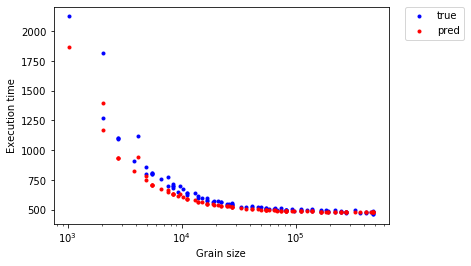
\includegraphics[scale=.4]{images/hpx_for_loop/blazemark/100000/marvin_pred_690_1.png}	
		\label{fig52:a}}
	\subfloat[]
	{\centering\includegraphics[scale=.4]{images/hpx_for_loop/blazemark/100000/marvin_pred_690_2.png}	
		\label{fig52:b}}\hfill
	\subfloat[]
	{\centering\includegraphics[scale=.4]{images/hpx_for_loop/blazemark/100000/marvin_pred_690_3.png}	
		\label{fig52:c}}
	\subfloat[]
	{\centering\includegraphics[scale=.4]{images/hpx_for_loop/blazemark/100000/marvin_pred_690_4.png}	
		\label{fig52:d}}\hfill
	\subfloat[]
	{\centering\includegraphics[scale=.4]{images/hpx_for_loop/blazemark/100000/marvin_pred_690_5.png}	
		\label{fig52:e}}
		\subfloat[]
	{\centering\includegraphics[scale=.4]{images/hpx_for_loop/blazemark/100000/marvin_pred_690_6.png}	
		\label{fig52:f}}\hfill
		\subfloat[]
	{\centering\includegraphics[scale=.4]{images/hpx_for_loop/blazemark/100000/marvin_pred_690_7.png}	
		\label{fig52:g}}
		\subfloat[]
	{\centering\includegraphics[scale=.4]{images/hpx_for_loop/blazemark/100000/marvin_pred_690_8.png}	
		\label{fig52:h}}
	\caption{The results of predicting execution time using the suggested analytical model with parameters identified using the parallel for-loop benchmark compared to the original values for $matrix\_{size}=690$, ran on (a) 1 core, (b) 2 cores, (c) 3 cores, (d) 4 cores, (e) 5 cores, (f) 6 cores, (g) 7 cores, and (h) 8 cores. The unit for execution time is microseconds.}
	\label{fig52}	
\end{figure}

\begin{figure}[H]
	\centering
	\subfloat[]
	{\centering\includegraphics[scale=.4]{images/hpx_for_loop/blazemark/100000/marvin_pred_4222_1.png}	
		\label{fig53:a}}
	\subfloat[]
	{\centering\includegraphics[scale=.4]{images/hpx_for_loop/blazemark/100000/marvin_pred_4222_2.png}	
		\label{fig53:b}}\hfill
	\subfloat[]
	{\centering\includegraphics[scale=.4]{images/hpx_for_loop/blazemark/100000/marvin_pred_4222_3.png}	
		\label{fig53:c}}
	\subfloat[]
	{\centering\includegraphics[scale=.4]{images/hpx_for_loop/blazemark/100000/marvin_pred_4222_4.png}	
		\label{fig53:d}}\hfill
	\subfloat[]
	{\centering\includegraphics[scale=.4]{images/hpx_for_loop/blazemark/100000/marvin_pred_4222_5.png}	
		\label{fig53:e}}
	\subfloat[]
	{\centering\includegraphics[scale=.4]{images/hpx_for_loop/blazemark/100000/marvin_pred_4222_6.png}	
		\label{fig53:f}}\hfill
	\subfloat[]
	{\centering\includegraphics[scale=.4]{images/hpx_for_loop/blazemark/100000/marvin_pred_4222_7.png}	
		\label{fig53:g}}
	\subfloat[]
	{\centering\includegraphics[scale=.4]{images/hpx_for_loop/blazemark/100000/marvin_pred_4222_8.png}	
		\label{fig53:h}}
	\caption{The results of predicting execution time using the suggested analytical model with parameters identified using the benchmark compared to the original values for $matrix\_{size}=4222$, ran on (a) 1 core, (b) 2 cores, (c) 3 cores, (d) 4 cores, (e) 5 cores, (f) 6 cores, (g) 7 cores, and (h) 8 cores. The unit for execution time is microseconds.}
	\label{fig53}	
\end{figure}

The $DMATDMATADD$ benchmark was run on $Marvin$ node with $Sandy\:Bridge$ architecture, with $256KB$ of level 2 cache, and $20MB$ of level 3 cache. In order for the $3$ same sized square matrices involved in $DMATDMATADD$ benchmark ($C=A+B$) to fit into level3 cache, they must be smaller than $935\times{935}$ in size. 

For matrix sizes greater than $935$, we observe an increase in execution time from our prediction using the proposed analytical model, as represented in Figure~\ref{fig53}. We have to pay a penalty for loading data from memory instead of cache.

Figure~\ref{fig54} shows the relative error, while Figure~\ref{fig55} represents the $R^2$ score both calculated for each specific number of cores individually, and for matrix sizes smaller than $935$.

\begin{figure}[H]
	\centering
	{\includegraphics[scale=.45]{images/hpx_for_loop/blazemark/100000000/marvin_relative_error_less_953.png}}
	\caption{The relative error of using the predicting the execution time based on grain size for the $DMATDMATADD$ benchmark from $Blazemark$ suite. The relative error of all matrix sizes smaller than $953$ was averaged for each specific number of cores.}\label{fig54}		
\end{figure}

\begin{figure}[H]
	\centering
	{\includegraphics[scale=.45]{images/hpx_for_loop/blazemark/100000000/marvin_r2_error_less_953.png}}
	\caption{The $R^2$ score of using the predicting the execution time based on grain size for the $DMATDMATADD$ benchmark from $Blazemark$ suite. The relative error of all matrix sizes smaller than $953$ was averaged for each specific number of cores.}\label{fig55}		
\end{figure}

Although we had completely ignored cache effects up until here for simplification, Figure~\ref{fig53} suggests that these effects do not influence the location of the flat region in the graph, which is the area with very small changes in execution time over which we observe the lowest execution time.   

Figure~\ref{fig56} shows the identified range for minimum execution time based on Formula~\ref{eq4}, for different matrix sizes ran on 8 cores.

\begin{figure}[H]
	\centering
	\subfloat[]
	{\centering\includegraphics[scale=.4]{images/hpx_for_loop/blazemark/100000/range/marvin_pred_690_8_10_500.png}	
		\label{fig56:a}}
	\subfloat[]
	{\centering\includegraphics[scale=.4]{images/hpx_for_loop/blazemark/100000/range/marvin_pred_912_8_10_500.png}	
		\label{fig56:b}}\hfill
	\subfloat[]
	{\centering\includegraphics[scale=.4]{images/hpx_for_loop/blazemark/100000/range/marvin_pred_1825_8_10_500.png}	
		\label{fig56:c}}
	\subfloat[]
	{\centering\includegraphics[scale=.4]{images/hpx_for_loop/blazemark/100000/range/marvin_pred_3193_8_10_500.png}	
		\label{fig56:d}}\hfill
	\subfloat[]
	{\centering\includegraphics[scale=.4]{images/hpx_for_loop/blazemark/100000/range/marvin_pred_4222_8_10_500.png}	
	\label{fig56:e}}
	{\centering\includegraphics[scale=.4]{images/hpx_for_loop/blazemark/100000/range/marvin_pred_4855_8_10_500.png}	
	\label{fig56:f}}
	{\centering\includegraphics[scale=.4]{images/hpx_for_loop/blazemark/100000/range/marvin_pred_6420_8_10_500.png}	
	\label{fig56:g}}
	\caption{The results of predicted values of execution time through curve fitting vs the real data for $matrix\_size=$, for (a) 690, (b) 912, (c) 1825, (d) 3193, (e) 4222, (f) 4855, (g) 6420, on 8 cores, with $\lambda_{s}=0.01$ and $\lambda_{b}=0.5$. The unit for execution time is microseconds.}
	\label{fig56}	
\end{figure}


\subsection{Predicting the Range of Chunk Size for Minimum Execution Time}
Having identified the range of minimum execution time for each matrix size, we can find the range of chunk size that would result in that range of grain size, for a specific block size.
As stated before, block size of $4\times{256}$ was selected as a safe choice for $DMATDMATADD$ benchmark. 


Figure~\ref{fig57} shows the identified range of chunk size for minimum execution time based on Formula~\ref{eq4}, for different matrix sizes ran on 8 cores, when $block\_{size}=4\times{256}$. Each point on the graph is the real data collected from running the $DMATDMATADD$ benchmarks. The red area denotes the proposed range for chunk size, and the red points are the data points that lie in this region. As it can be seen the predicted range for chunk size are reasonable.   

\begin{figure}[H]
	\centering
	\subfloat[]
	{\centering\includegraphics[scale=.4]{images/hpx_for_loop/blazemark/100000/chunk_sizes/marvin_pred_690_8_10_500_5_21.png}	
		\label{fig57:a}}
	\subfloat[]
	{\centering\includegraphics[scale=.4]{images/hpx_for_loop/blazemark/100000/chunk_sizes/marvin_pred_912_8_10_500_6_37.png}	
		\label{fig57:b}}\hfill
	\subfloat[]
	 {\centering\includegraphics[scale=.4]{images/hpx_for_loop/blazemark/100000/chunk_sizes/marvin_pred_1825_8_10_500_12_152.png}	
		\label{fig57:c}}
	\subfloat[]
	{\centering\includegraphics[scale=.4]{images/hpx_for_loop/blazemark/100000/chunk_sizes/marvin_pred_3193_8_10_500_19_432.png}	
		\label{fig57:d}}\hfill
	\subfloat[]
	{\centering\includegraphics[scale=.4]{images/hpx_for_loop/blazemark/100000/chunk_sizes/marvin_pred_4222_8_10_500_25_747.png}	
		\label{fig57:e}}
	{\centering\includegraphics[scale=.4]{images/hpx_for_loop/blazemark/100000/chunk_sizes/marvin_pred_4855_8_10_500_28_960.png}	
		\label{fig57:f}}
	{\centering\includegraphics[scale=.4]{images/hpx_for_loop/blazemark/100000/chunk_sizes/marvin_pred_6420_8_10_500_38_1737.png}	
		\label{fig57:g}}
	\caption{The suggested range of chunk size for minimum execution time with $block\_{size}=4\times{256}$, for $matrix\_size=$, for (a) 690, (b) 912, (c) 1825, (d) 3193, (e) 4222, (f) 4855, (g) 6420, on 8 cores, when $\lambda_{s}=0.5$ and $\lambda_{b}=0.01$. The unit for execution time is microseconds.}
	\label{fig57}	
\end{figure}


\section{Conclusion}
In the previous sections we offered an analytical model to predict the behavior of execution time in terms grain size for a balanced parallel loop, and based on that model suggested a method to estimate the range of grain size to ensure staying in the flat region of the bathtub curve of execution time. The proposed model was then validated using a simple implemented benchmark. The parameters found through the benchmark was then utilized to predict the execution time of the $DMATDMATADD$ benchmark from $Blazemark$ suite. We were also able to find the range of grain size to achieve minimum execution time. 
At this point by selecting a reasonable value for block size, the range of chunk size to ensure staying in that range of grain size could be identified.

We propose to run the parallel for-loop benchmark in Listing~\ref{hpx_for_loop} for a reasonable \emph{problem\_{size} = 100000}, with different values for chunk size on different number of cores, and use the collected data to estimate the $\alpha$ and $\sigma$ parameters through curve fitting. This process could be added as an extra step to building process of Blaze. 
The complexity of the expression to be evaluated is then calculated at compile time as the number of floating point operations. 
A block size should also be selected based on the available cache size, the cache line, and the number of matrices involved in the operation. This part could also be done at compile time.   
At runtime, based on the matrix size and number of cores chosen to run the program on, the range of chunk size to achieve the lowest execution time for each specific expression is identified.

It has to be mentioned that although the proposed formula for execution time vs grain size depends on the sequential execution time, the proposed range for minimum execution time does not rely on sequential execution time, but depends on total amount of work, number of cores, overhead of creating and managing tasks, and the values we choose for the threshold on both sides($\lambda_{b}$ and $\lambda_{s}$).
 


%\vspace{\baselineskip}
%\subsection{Analyzing the Data}
%Throughout these experiments we try to fix or eliminate the factors we believe will affect the execution time as much as possible, study the results, and then introduce one factor to the model and study the behavior of the model. 



\vspace{\baselineskip}
%\subsection{Step 1: Sequential Run}
%In the first step in order to eliminate all the factors related to parallel execution we run the code sequentially for some problem sizes. The obtained result, as shown in Figure~\ref{fig26} demonstrates an overhead that increases as the number of iterations increases.
%
%\begin{figure}
%	\centering
%	\includegraphics[width=1\linewidth]{images/hpx_for_loop/overheads_seq.png}
%	\caption{The results obtained from running the hpx for loop sequentially}	
%	\label{fig26}
%\end{figure}




\vspace{\baselineskip}

\clearpage

%\subsection{Step 1: Single-task, single-core runs}
%At the first step, we look at the cases where only one task has been created, the program is run on only one core. This problem could be assumed to be equivalent to running the same amount of work sequentially with an additional cost of creating just one task. 
%\subsubsection{Expected Model}
%With this assumption we expect the execution time to be summation of the time it takes to perform the total amount of work(\textit{problem\textunderscore{size}}) and the overhead of creating one HPX task($\alpha$). Formula~\ref{chunk1} shows the expected formula.
%
%\begin{equation}\label{chunk1}
%execution\:\:time = \alpha + problem\:\:size
%\end{equation}  
%
%\vspace{\baselineskip}
%\subsubsection{Original Data}
%In order to check our proposed model for this simplified problem, we collected data from running the program, setting the \textit{chunk\textunderscore{size}} to 1, \textit{num\textunderscore{iterations}} to 1, and changing the \textit{iter\textunderscore{length}} from 1 to 10,000,000. 




%To summarize, knowing the grain size, we are expecting the execution time in a many-task runtime system to be mainly affected by these factors, the overhead of creating one task($\alpha$), the number of cores that are actually doing the work($M$), the sequential execution time($t_s$), and finally the portion of the program that could actually be parallelized($\sigma$). 
%
%If we try to integrate these information into a formula, we would expect the relation between execution time($t$) and number of tasks($n_t$) as follows:
%\begin{equation}\label{new1}
%t=\frac{\alpha{n_t}+t_s}{M}+\sigma
%\end{equation}
%
%which could be decomposed into these two equations:
%
%
%Now we use this function to find the best three parameters $\alpha$, $t_s$, and $\sigma$ so that the collected data would fit this model. For this purpose we used the \textit{curve\textunderscore{fit}} package from \textit{SciPy} library in \textit{python}.
%
%In order to make Equation~\ref{new1} differentiable, we used the softplus function(Equation~\ref{softplus1}) to represent $M$ based on $n_t$.
%\begin{equation}\label{softplus1}
%f(x)=Ln(1+e^x)
%\end{equation}
%
%Which results in Equation~\ref{soft_plus1}:
%\begin{equation}\label{soft_plus1}
%t=\frac{\alpha{n_t}+t_s}{(N-1)-Ln(1+(e^{N-1}-1)e^{-n_t})}+\sigma
%\end{equation}




\vspace{\baselineskip}